% Options for packages loaded elsewhere
\PassOptionsToPackage{unicode}{hyperref}
\PassOptionsToPackage{hyphens}{url}
\PassOptionsToPackage{dvipsnames,svgnames,x11names}{xcolor}
%
\documentclass[
  letterpaper,
  DIV=11,
  numbers=noendperiod]{scrartcl}

\usepackage{amsmath,amssymb}
\usepackage{lmodern}
\usepackage{iftex}
\ifPDFTeX
  \usepackage[T1]{fontenc}
  \usepackage[utf8]{inputenc}
  \usepackage{textcomp} % provide euro and other symbols
\else % if luatex or xetex
  \usepackage{unicode-math}
  \defaultfontfeatures{Scale=MatchLowercase}
  \defaultfontfeatures[\rmfamily]{Ligatures=TeX,Scale=1}
\fi
% Use upquote if available, for straight quotes in verbatim environments
\IfFileExists{upquote.sty}{\usepackage{upquote}}{}
\IfFileExists{microtype.sty}{% use microtype if available
  \usepackage[]{microtype}
  \UseMicrotypeSet[protrusion]{basicmath} % disable protrusion for tt fonts
}{}
\makeatletter
\@ifundefined{KOMAClassName}{% if non-KOMA class
  \IfFileExists{parskip.sty}{%
    \usepackage{parskip}
  }{% else
    \setlength{\parindent}{0pt}
    \setlength{\parskip}{6pt plus 2pt minus 1pt}}
}{% if KOMA class
  \KOMAoptions{parskip=half}}
\makeatother
\usepackage{xcolor}
\setlength{\emergencystretch}{3em} % prevent overfull lines
\setcounter{secnumdepth}{-\maxdimen} % remove section numbering
% Make \paragraph and \subparagraph free-standing
\ifx\paragraph\undefined\else
  \let\oldparagraph\paragraph
  \renewcommand{\paragraph}[1]{\oldparagraph{#1}\mbox{}}
\fi
\ifx\subparagraph\undefined\else
  \let\oldsubparagraph\subparagraph
  \renewcommand{\subparagraph}[1]{\oldsubparagraph{#1}\mbox{}}
\fi

\usepackage{color}
\usepackage{fancyvrb}
\newcommand{\VerbBar}{|}
\newcommand{\VERB}{\Verb[commandchars=\\\{\}]}
\DefineVerbatimEnvironment{Highlighting}{Verbatim}{commandchars=\\\{\}}
% Add ',fontsize=\small' for more characters per line
\usepackage{framed}
\definecolor{shadecolor}{RGB}{241,243,245}
\newenvironment{Shaded}{\begin{snugshade}}{\end{snugshade}}
\newcommand{\AlertTok}[1]{\textcolor[rgb]{0.68,0.00,0.00}{#1}}
\newcommand{\AnnotationTok}[1]{\textcolor[rgb]{0.37,0.37,0.37}{#1}}
\newcommand{\AttributeTok}[1]{\textcolor[rgb]{0.40,0.45,0.13}{#1}}
\newcommand{\BaseNTok}[1]{\textcolor[rgb]{0.68,0.00,0.00}{#1}}
\newcommand{\BuiltInTok}[1]{\textcolor[rgb]{0.00,0.23,0.31}{#1}}
\newcommand{\CharTok}[1]{\textcolor[rgb]{0.13,0.47,0.30}{#1}}
\newcommand{\CommentTok}[1]{\textcolor[rgb]{0.37,0.37,0.37}{#1}}
\newcommand{\CommentVarTok}[1]{\textcolor[rgb]{0.37,0.37,0.37}{\textit{#1}}}
\newcommand{\ConstantTok}[1]{\textcolor[rgb]{0.56,0.35,0.01}{#1}}
\newcommand{\ControlFlowTok}[1]{\textcolor[rgb]{0.00,0.23,0.31}{#1}}
\newcommand{\DataTypeTok}[1]{\textcolor[rgb]{0.68,0.00,0.00}{#1}}
\newcommand{\DecValTok}[1]{\textcolor[rgb]{0.68,0.00,0.00}{#1}}
\newcommand{\DocumentationTok}[1]{\textcolor[rgb]{0.37,0.37,0.37}{\textit{#1}}}
\newcommand{\ErrorTok}[1]{\textcolor[rgb]{0.68,0.00,0.00}{#1}}
\newcommand{\ExtensionTok}[1]{\textcolor[rgb]{0.00,0.23,0.31}{#1}}
\newcommand{\FloatTok}[1]{\textcolor[rgb]{0.68,0.00,0.00}{#1}}
\newcommand{\FunctionTok}[1]{\textcolor[rgb]{0.28,0.35,0.67}{#1}}
\newcommand{\ImportTok}[1]{\textcolor[rgb]{0.00,0.46,0.62}{#1}}
\newcommand{\InformationTok}[1]{\textcolor[rgb]{0.37,0.37,0.37}{#1}}
\newcommand{\KeywordTok}[1]{\textcolor[rgb]{0.00,0.23,0.31}{#1}}
\newcommand{\NormalTok}[1]{\textcolor[rgb]{0.00,0.23,0.31}{#1}}
\newcommand{\OperatorTok}[1]{\textcolor[rgb]{0.37,0.37,0.37}{#1}}
\newcommand{\OtherTok}[1]{\textcolor[rgb]{0.00,0.23,0.31}{#1}}
\newcommand{\PreprocessorTok}[1]{\textcolor[rgb]{0.68,0.00,0.00}{#1}}
\newcommand{\RegionMarkerTok}[1]{\textcolor[rgb]{0.00,0.23,0.31}{#1}}
\newcommand{\SpecialCharTok}[1]{\textcolor[rgb]{0.37,0.37,0.37}{#1}}
\newcommand{\SpecialStringTok}[1]{\textcolor[rgb]{0.13,0.47,0.30}{#1}}
\newcommand{\StringTok}[1]{\textcolor[rgb]{0.13,0.47,0.30}{#1}}
\newcommand{\VariableTok}[1]{\textcolor[rgb]{0.07,0.07,0.07}{#1}}
\newcommand{\VerbatimStringTok}[1]{\textcolor[rgb]{0.13,0.47,0.30}{#1}}
\newcommand{\WarningTok}[1]{\textcolor[rgb]{0.37,0.37,0.37}{\textit{#1}}}

\providecommand{\tightlist}{%
  \setlength{\itemsep}{0pt}\setlength{\parskip}{0pt}}\usepackage{longtable,booktabs,array}
\usepackage{calc} % for calculating minipage widths
% Correct order of tables after \paragraph or \subparagraph
\usepackage{etoolbox}
\makeatletter
\patchcmd\longtable{\par}{\if@noskipsec\mbox{}\fi\par}{}{}
\makeatother
% Allow footnotes in longtable head/foot
\IfFileExists{footnotehyper.sty}{\usepackage{footnotehyper}}{\usepackage{footnote}}
\makesavenoteenv{longtable}
\usepackage{graphicx}
\makeatletter
\def\maxwidth{\ifdim\Gin@nat@width>\linewidth\linewidth\else\Gin@nat@width\fi}
\def\maxheight{\ifdim\Gin@nat@height>\textheight\textheight\else\Gin@nat@height\fi}
\makeatother
% Scale images if necessary, so that they will not overflow the page
% margins by default, and it is still possible to overwrite the defaults
% using explicit options in \includegraphics[width, height, ...]{}
\setkeys{Gin}{width=\maxwidth,height=\maxheight,keepaspectratio}
% Set default figure placement to htbp
\makeatletter
\def\fps@figure{htbp}
\makeatother

\KOMAoption{captions}{tableheading}
\makeatletter
\makeatother
\makeatletter
\makeatother
\makeatletter
\@ifpackageloaded{caption}{}{\usepackage{caption}}
\AtBeginDocument{%
\ifdefined\contentsname
  \renewcommand*\contentsname{Table of contents}
\else
  \newcommand\contentsname{Table of contents}
\fi
\ifdefined\listfigurename
  \renewcommand*\listfigurename{List of Figures}
\else
  \newcommand\listfigurename{List of Figures}
\fi
\ifdefined\listtablename
  \renewcommand*\listtablename{List of Tables}
\else
  \newcommand\listtablename{List of Tables}
\fi
\ifdefined\figurename
  \renewcommand*\figurename{Figure}
\else
  \newcommand\figurename{Figure}
\fi
\ifdefined\tablename
  \renewcommand*\tablename{Table}
\else
  \newcommand\tablename{Table}
\fi
}
\@ifpackageloaded{float}{}{\usepackage{float}}
\floatstyle{ruled}
\@ifundefined{c@chapter}{\newfloat{codelisting}{h}{lop}}{\newfloat{codelisting}{h}{lop}[chapter]}
\floatname{codelisting}{Listing}
\newcommand*\listoflistings{\listof{codelisting}{List of Listings}}
\makeatother
\makeatletter
\@ifpackageloaded{caption}{}{\usepackage{caption}}
\@ifpackageloaded{subcaption}{}{\usepackage{subcaption}}
\makeatother
\makeatletter
\@ifpackageloaded{tcolorbox}{}{\usepackage[many]{tcolorbox}}
\makeatother
\makeatletter
\@ifundefined{shadecolor}{\definecolor{shadecolor}{rgb}{.97, .97, .97}}
\makeatother
\makeatletter
\makeatother
\ifLuaTeX
  \usepackage{selnolig}  % disable illegal ligatures
\fi
\IfFileExists{bookmark.sty}{\usepackage{bookmark}}{\usepackage{hyperref}}
\IfFileExists{xurl.sty}{\usepackage{xurl}}{} % add URL line breaks if available
\urlstyle{same} % disable monospaced font for URLs
\hypersetup{
  pdftitle={Surfclam\_growth\_Sep22\_Dec22},
  colorlinks=true,
  linkcolor={blue},
  filecolor={Maroon},
  citecolor={Blue},
  urlcolor={Blue},
  pdfcreator={LaTeX via pandoc}}

\title{Surfclam\_growth\_Sep22\_Dec22}
\author{}
\date{}

\begin{document}
\maketitle
\ifdefined\Shaded\renewenvironment{Shaded}{\begin{tcolorbox}[sharp corners, interior hidden, frame hidden, borderline west={3pt}{0pt}{shadecolor}, boxrule=0pt, enhanced, breakable]}{\end{tcolorbox}}\fi

\begin{Shaded}
\begin{Highlighting}[]
\DocumentationTok{\#\#{-}{-}{-}{-}{-}{-}{-}{-}{-}{-}{-}{-}{-}{-}{-}{-}{-}{-}{-}{-}{-}{-}{-}{-}{-}{-}{-}{-}{-}{-}{-}{-}{-}{-}{-}{-}}
\DocumentationTok{\#\#  Sep to Dec growth accounting  {-}{-}}
\DocumentationTok{\#\#{-}{-}{-}{-}{-}{-}{-}{-}{-}{-}{-}{-}{-}{-}{-}{-}{-}{-}{-}{-}{-}{-}{-}{-}{-}{-}{-}{-}{-}{-}{-}{-}{-}{-}{-}{-}}

\NormalTok{growth\_dec }\OtherTok{\textless{}{-}}\NormalTok{ growth[growth}\SpecialCharTok{$}\NormalTok{Collection.month}\SpecialCharTok{==}\StringTok{"December"}\NormalTok{,]}

\FunctionTok{head}\NormalTok{(growth\_dec)}
\end{Highlighting}
\end{Shaded}

\begin{verbatim}
   Start_date     Site Treatment Buried_Dec Location_code color.1 color.2  X
30  9/26/2022 Eel Pond         S          N            B1       R         NA
31  9/26/2022 Eel Pond         S          N            B1       Y         NA
32  9/26/2022 Eel Pond         S          N            B1       B         NA
33  9/26/2022 Eel Pond         S          N            B1       L         NA
34  9/26/2022 Eel Pond         S          N            B1       R       Y NA
35  9/26/2022 Eel Pond         S          N            B1       R       B NA
   Start_len_mm Start_height_mm Start_thickness_mm Collection.month
30        18.21           14.00               8.10         December
31        12.71            9.63               5.56         December
32        12.80            9.09               4.92         December
33        11.23            8.83               4.91         December
34        10.59            8.21               4.42         December
35         9.94            7.47               4.03         December
   Collection1_date Elapsed_days depth_cm color L_mm H_mm T_mm growth_marking
30        12/5/2022           70       4+     R   NA   NA   NA           10.1
31        12/5/2022           70                  NA   NA   NA             NA
32        12/5/2022           70       4+     B   NA   NA   NA             NA
33        12/5/2022           70                  NA   NA   NA             NA
34        12/5/2022           70                  NA   NA   NA             NA
35        12/5/2022           70                  NA   NA   NA             NA
   Dead_lengths_mm growth_height growth_marking_perc_error notes AliveOrDead
30           18.13            NA                        NA              Dead
31              NA            NA                        NA           Missing
32              NA            NA                        NA           Missing
33              NA            NA                        NA           Missing
34              NA            NA                        NA           Missing
35              NA            NA                        NA           Missing
   len_tot len_per_day height_tot height_per_day
30      NA          NA         NA             NA
31      NA          NA         NA             NA
32      NA          NA         NA             NA
33      NA          NA         NA             NA
34      NA          NA         NA             NA
35      NA          NA         NA             NA
\end{verbatim}

\begin{Shaded}
\begin{Highlighting}[]
\FunctionTok{str}\NormalTok{(growth\_dec)}
\end{Highlighting}
\end{Shaded}

\begin{verbatim}
'data.frame':   188 obs. of  29 variables:
 $ Start_date               : chr  "9/26/2022" "9/26/2022" "9/26/2022" "9/26/2022" ...
 $ Site                     : chr  "Eel Pond" "Eel Pond" "Eel Pond" "Eel Pond" ...
 $ Treatment                : chr  "S" "S" "S" "S" ...
 $ Buried_Dec               : chr  "N" "N" "N" "N" ...
 $ Location_code            : chr  "B1" "B1" "B1" "B1" ...
 $ color.1                  : chr  "R" "Y" "B" "L" ...
 $ color.2                  : chr  "" "" "" "" ...
 $ X                        : logi  NA NA NA NA NA NA ...
 $ Start_len_mm             : num  18.2 12.7 12.8 11.2 10.6 ...
 $ Start_height_mm          : num  14 9.63 9.09 8.83 8.21 ...
 $ Start_thickness_mm       : num  8.1 5.56 4.92 4.91 4.42 ...
 $ Collection.month         : chr  "December" "December" "December" "December" ...
 $ Collection1_date         : chr  "12/5/2022" "12/5/2022" "12/5/2022" "12/5/2022" ...
 $ Elapsed_days             : int  70 70 70 70 70 70 70 70 70 70 ...
 $ depth_cm                 : chr  "4+" "" "4+" "" ...
 $ color                    : chr  "R" "" "B" "" ...
 $ L_mm                     : num  NA NA NA NA NA NA NA NA NA NA ...
 $ H_mm                     : num  NA NA NA NA NA NA NA NA NA NA ...
 $ T_mm                     : num  NA NA NA NA NA NA NA NA NA NA ...
 $ growth_marking           : num  10.1 NA NA NA NA NA NA NA NA 7.67 ...
 $ Dead_lengths_mm          : num  18.1 NA NA NA NA ...
 $ growth_height            : num  NA NA NA NA NA NA NA NA NA NA ...
 $ growth_marking_perc_error: num  NA NA NA NA NA NA NA NA NA NA ...
 $ notes                    : chr  "" "" "" "" ...
 $ AliveOrDead              : chr  "Dead" "Missing" "Missing" "Missing" ...
 $ len_tot                  : num  NA NA NA NA NA NA NA NA NA NA ...
 $ len_per_day              : num  NA NA NA NA NA NA NA NA NA NA ...
 $ height_tot               : num  NA NA NA NA NA NA NA NA NA NA ...
 $ height_per_day           : num  NA NA NA NA NA NA NA NA NA NA ...
\end{verbatim}

\begin{Shaded}
\begin{Highlighting}[]
\NormalTok{growth\_dec}\SpecialCharTok{$}\NormalTok{Site }\OtherTok{\textless{}{-}} \FunctionTok{as.factor}\NormalTok{(growth\_dec}\SpecialCharTok{$}\NormalTok{Site)}
\NormalTok{growth\_dec}\SpecialCharTok{$}\NormalTok{Treatment }\OtherTok{\textless{}{-}} \FunctionTok{as.factor}\NormalTok{(growth\_dec}\SpecialCharTok{$}\NormalTok{Treatment)}
\NormalTok{growth\_dec}\SpecialCharTok{$}\NormalTok{AliveOrDead }\OtherTok{\textless{}{-}} \FunctionTok{as.factor}\NormalTok{(growth\_dec}\SpecialCharTok{$}\NormalTok{AliveOrDead)}


\CommentTok{\#Length change through December}
\NormalTok{ growth\_dec\_no\_na }\OtherTok{\textless{}{-}}\NormalTok{ growth\_dec[}\SpecialCharTok{!}\FunctionTok{is.na}\NormalTok{(growth\_dec}\SpecialCharTok{$}\NormalTok{len\_tot),]}

\NormalTok{ mod\_growth\_full }\OtherTok{\textless{}{-}} \FunctionTok{lme}\NormalTok{(len\_tot}\SpecialCharTok{\textasciitilde{}}\NormalTok{Treatment}\SpecialCharTok{*}\NormalTok{Site}\SpecialCharTok{+}\NormalTok{Start\_len\_mm}\SpecialCharTok{+}\NormalTok{Start\_len\_mm}\SpecialCharTok{:}\NormalTok{Site, }
                        \AttributeTok{random =} \SpecialCharTok{\textasciitilde{}}\DecValTok{1}\SpecialCharTok{|}\NormalTok{Location\_code, }\AttributeTok{data =}\NormalTok{ growth\_dec\_no\_na)}
  \FunctionTok{summary}\NormalTok{(mod\_growth\_full)}
\end{Highlighting}
\end{Shaded}

\begin{verbatim}
Linear mixed-effects model fit by REML
  Data: growth_dec_no_na 
       AIC      BIC    logLik
  392.5676 412.5661 -188.2838

Random effects:
 Formula: ~1 | Location_code
        (Intercept) Residual
StdDev:   0.5143511 1.694901

Fixed effects:  len_tot ~ Treatment * Site + Start_len_mm + Start_len_mm:Site 
                           Value Std.Error DF    t-value p-value
(Intercept)             6.267963  2.619019 78  2.3932488  0.0191
TreatmentS             -0.834806  0.665629 78 -1.2541600  0.2135
SitePtown               6.212703  3.191472 78  1.9466575  0.0552
Start_len_mm            0.028340  0.220924 78  0.1282803  0.8983
TreatmentS:SitePtown    0.430041  0.842145 78  0.5106497  0.6110
SitePtown:Start_len_mm -0.135411  0.272019 78 -0.4977989  0.6200
 Correlation: 
                       (Intr) TrtmnS StPtwn Strt__ TrS:SP
TreatmentS             -0.225                            
SitePtown              -0.822  0.179                     
Start_len_mm           -0.981  0.080  0.811              
TreatmentS:SitePtown    0.176 -0.741 -0.219 -0.078       
SitePtown:Start_len_mm  0.797 -0.067 -0.982 -0.812  0.077

Standardized Within-Group Residuals:
       Min         Q1        Med         Q3        Max 
-3.1526673 -0.4472383 -0.0421636  0.4210455  5.2736643 

Number of Observations: 96
Number of Groups: 13 
\end{verbatim}

\begin{Shaded}
\begin{Highlighting}[]
\NormalTok{  M\_int}\OtherTok{\textless{}{-}}\FunctionTok{update}\NormalTok{(mod\_growth\_full, .}\SpecialCharTok{\textasciitilde{}}\NormalTok{. }\SpecialCharTok{{-}}\NormalTok{ Start\_len\_mm}\SpecialCharTok{:}\NormalTok{Site)}
\NormalTok{  M }\OtherTok{\textless{}{-}} \FunctionTok{update}\NormalTok{(M\_int, }\SpecialCharTok{\textasciitilde{}}\NormalTok{. }\SpecialCharTok{{-}}\NormalTok{ Treatment}\SpecialCharTok{:}\NormalTok{Site)}
\NormalTok{  M2 }\OtherTok{\textless{}{-}} \FunctionTok{update}\NormalTok{(M\_int, }\SpecialCharTok{\textasciitilde{}}\NormalTok{. }\SpecialCharTok{{-}}\NormalTok{ Start\_len\_mm)}
  
  \FunctionTok{summary}\NormalTok{(M\_int)}
\end{Highlighting}
\end{Shaded}

\begin{verbatim}
Linear mixed-effects model fit by REML
  Data: growth_dec_no_na 
       AIC      BIC    logLik
  390.0454 407.6215 -188.0227

Random effects:
 Formula: ~1 | Location_code
        (Intercept) Residual
StdDev:     0.52496 1.686073

Fixed effects:  len_tot ~ Treatment + Site + Start_len_mm + Treatment:Site 
                         Value Std.Error DF   t-value p-value
(Intercept)           7.309081 1.5750050 79  4.640672  0.0000
TreatmentS           -0.855702 0.6649536 79 -1.286859  0.2019
SitePtown             4.651195 0.6096603 79  7.629158  0.0000
Start_len_mm         -0.061376 0.1282481 79 -0.478576  0.6336
TreatmentS:SitePtown  0.467173 0.8400777 79  0.556107  0.5797
 Correlation: 
                     (Intr) TrtmnS StPtwn Strt__
TreatmentS           -0.286                     
SitePtown            -0.345  0.595              
Start_len_mm         -0.946  0.044  0.121       
TreatmentS:SitePtown  0.190 -0.739 -0.750 -0.027

Standardized Within-Group Residuals:
        Min          Q1         Med          Q3         Max 
-3.24136962 -0.44821774 -0.02818898  0.43585381  5.29828093 

Number of Observations: 96
Number of Groups: 13 
\end{verbatim}

\begin{Shaded}
\begin{Highlighting}[]
  \FunctionTok{summary}\NormalTok{(M)}
\end{Highlighting}
\end{Shaded}

\begin{verbatim}
Linear mixed-effects model fit by REML
  Data: growth_dec_no_na 
       AIC      BIC    logLik
  389.8005 404.9312 -188.9002

Random effects:
 Formula: ~1 | Location_code
        (Intercept) Residual
StdDev:   0.4412753 1.691199

Fixed effects:  len_tot ~ Treatment + Site + Start_len_mm 
                 Value Std.Error DF   t-value p-value
(Intercept)   7.134162 1.5398563 80  4.633005  0.0000
TreatmentS   -0.610199 0.4256156 80 -1.433685  0.1556
SitePtown     4.905660 0.3930735 80 12.480263  0.0000
Start_len_mm -0.056663 0.1282433 80 -0.441838  0.6598
 Correlation: 
             (Intr) TrtmnS StPtwn
TreatmentS   -0.210              
SitePtown    -0.307  0.072       
Start_len_mm -0.963  0.037  0.153

Standardized Within-Group Residuals:
        Min          Q1         Med          Q3         Max 
-3.27627185 -0.44522470 -0.04230813  0.40510889  5.35029526 

Number of Observations: 96
Number of Groups: 13 
\end{verbatim}

\begin{Shaded}
\begin{Highlighting}[]
  \FunctionTok{summary}\NormalTok{(M2)}
\end{Highlighting}
\end{Shaded}

\begin{verbatim}
Linear mixed-effects model fit by REML
  Data: growth_dec_no_na 
       AIC      BIC    logLik
  386.0006 401.1314 -187.0003

Random effects:
 Formula: ~1 | Location_code
        (Intercept) Residual
StdDev:   0.5106636 1.680681

Fixed effects:  len_tot ~ Treatment + Site + Treatment:Site 
                         Value Std.Error DF   t-value p-value
(Intercept)           6.598488 0.5057290 80 13.047479  0.0000
TreatmentS           -0.843044 0.6581080 80 -1.281012  0.2039
SitePtown             4.688304 0.6010795 80  7.799808  0.0000
TreatmentS:SitePtown  0.451659 0.8325155 80  0.542523  0.5890
 Correlation: 
                     (Intr) TrtmnS StPtwn
TreatmentS           -0.756              
SitePtown            -0.719  0.594       
TreatmentS:SitePtown  0.510 -0.740 -0.753

Standardized Within-Group Residuals:
        Min          Q1         Med          Q3         Max 
-3.20764432 -0.44920300 -0.03618056  0.43758754  5.32151595 

Number of Observations: 96
Number of Groups: 13 
\end{verbatim}

\begin{Shaded}
\begin{Highlighting}[]
\FunctionTok{AIC}\NormalTok{(mod\_growth\_full,M\_int,M,M2)}
\end{Highlighting}
\end{Shaded}

\begin{verbatim}
Warning in AIC.default(mod_growth_full, M_int, M, M2): models are not all fitted
to the same number of observations
\end{verbatim}

\begin{verbatim}
                df      AIC
mod_growth_full  8 392.5676
M_int            7 390.0454
M                6 389.8005
M2               6 386.0006
\end{verbatim}

\begin{Shaded}
\begin{Highlighting}[]
\FunctionTok{str}\NormalTok{(growth\_dec)}
\end{Highlighting}
\end{Shaded}

\begin{verbatim}
'data.frame':   188 obs. of  29 variables:
 $ Start_date               : chr  "9/26/2022" "9/26/2022" "9/26/2022" "9/26/2022" ...
 $ Site                     : Factor w/ 2 levels "Eel Pond","Ptown": 1 1 1 1 1 1 1 1 1 1 ...
 $ Treatment                : Factor w/ 2 levels "N","S": 2 2 2 2 2 2 2 2 2 2 ...
 $ Buried_Dec               : chr  "N" "N" "N" "N" ...
 $ Location_code            : chr  "B1" "B1" "B1" "B1" ...
 $ color.1                  : chr  "R" "Y" "B" "L" ...
 $ color.2                  : chr  "" "" "" "" ...
 $ X                        : logi  NA NA NA NA NA NA ...
 $ Start_len_mm             : num  18.2 12.7 12.8 11.2 10.6 ...
 $ Start_height_mm          : num  14 9.63 9.09 8.83 8.21 ...
 $ Start_thickness_mm       : num  8.1 5.56 4.92 4.91 4.42 ...
 $ Collection.month         : chr  "December" "December" "December" "December" ...
 $ Collection1_date         : chr  "12/5/2022" "12/5/2022" "12/5/2022" "12/5/2022" ...
 $ Elapsed_days             : int  70 70 70 70 70 70 70 70 70 70 ...
 $ depth_cm                 : chr  "4+" "" "4+" "" ...
 $ color                    : chr  "R" "" "B" "" ...
 $ L_mm                     : num  NA NA NA NA NA NA NA NA NA NA ...
 $ H_mm                     : num  NA NA NA NA NA NA NA NA NA NA ...
 $ T_mm                     : num  NA NA NA NA NA NA NA NA NA NA ...
 $ growth_marking           : num  10.1 NA NA NA NA NA NA NA NA 7.67 ...
 $ Dead_lengths_mm          : num  18.1 NA NA NA NA ...
 $ growth_height            : num  NA NA NA NA NA NA NA NA NA NA ...
 $ growth_marking_perc_error: num  NA NA NA NA NA NA NA NA NA NA ...
 $ notes                    : chr  "" "" "" "" ...
 $ AliveOrDead              : Factor w/ 3 levels "Alive","Dead",..: 2 3 3 3 3 3 3 3 3 2 ...
 $ len_tot                  : num  NA NA NA NA NA NA NA NA NA NA ...
 $ len_per_day              : num  NA NA NA NA NA NA NA NA NA NA ...
 $ height_tot               : num  NA NA NA NA NA NA NA NA NA NA ...
 $ height_per_day           : num  NA NA NA NA NA NA NA NA NA NA ...
\end{verbatim}

\begin{Shaded}
\begin{Highlighting}[]
\NormalTok{mod\_growth\_full }\OtherTok{\textless{}{-}} \FunctionTok{lme}\NormalTok{(height\_tot}\SpecialCharTok{\textasciitilde{}}\NormalTok{Treatment}\SpecialCharTok{*}\NormalTok{Site}\SpecialCharTok{+}\NormalTok{Start\_len\_mm}\SpecialCharTok{+}\NormalTok{Start\_len\_mm}\SpecialCharTok{:}\NormalTok{Site, }
                       \AttributeTok{random =} \SpecialCharTok{\textasciitilde{}}\DecValTok{1}\SpecialCharTok{|}\NormalTok{Location\_code, }\AttributeTok{data =}\NormalTok{ growth\_dec\_no\_na)}
\FunctionTok{summary}\NormalTok{(mod\_growth\_full)}
\end{Highlighting}
\end{Shaded}

\begin{verbatim}
Linear mixed-effects model fit by REML
  Data: growth_dec_no_na 
       AIC     BIC    logLik
  332.1825 352.181 -158.0913

Random effects:
 Formula: ~1 | Location_code
        (Intercept) Residual
StdDev:   0.3949829  1.20796

Fixed effects:  height_tot ~ Treatment * Site + Start_len_mm + Start_len_mm:Site 
                           Value Std.Error DF    t-value p-value
(Intercept)             4.776407 1.8703008 78  2.5538178  0.0126
TreatmentS             -0.684389 0.4835292 78 -1.4154028  0.1609
SitePtown               4.705827 2.2798269 78  2.0641157  0.0423
Start_len_mm            0.040310 0.1576712 78  0.2556597  0.7989
TreatmentS:SitePtown    0.539834 0.6105211 78  0.8842177  0.3793
SitePtown:Start_len_mm -0.090582 0.1941359 78 -0.4665926  0.6421
 Correlation: 
                       (Intr) TrtmnS StPtwn Strt__ TrS:SP
TreatmentS             -0.225                            
SitePtown              -0.822  0.179                     
Start_len_mm           -0.980  0.078  0.811              
TreatmentS:SitePtown    0.175 -0.737 -0.220 -0.078       
SitePtown:Start_len_mm  0.797 -0.065 -0.981 -0.812  0.077

Standardized Within-Group Residuals:
        Min          Q1         Med          Q3         Max 
-3.37401820 -0.48124421 -0.01575827  0.42648795  5.25895442 

Number of Observations: 96
Number of Groups: 13 
\end{verbatim}

\begin{Shaded}
\begin{Highlighting}[]
\NormalTok{M\_int}\OtherTok{\textless{}{-}}\FunctionTok{update}\NormalTok{(mod\_growth\_full, .}\SpecialCharTok{\textasciitilde{}}\NormalTok{. }\SpecialCharTok{{-}}\NormalTok{ Start\_len\_mm}\SpecialCharTok{:}\NormalTok{Site)}
\NormalTok{M }\OtherTok{\textless{}{-}} \FunctionTok{update}\NormalTok{(M\_int, }\SpecialCharTok{\textasciitilde{}}\NormalTok{. }\SpecialCharTok{{-}}\NormalTok{ Treatment}\SpecialCharTok{:}\NormalTok{Site)}
\NormalTok{M2 }\OtherTok{\textless{}{-}} \FunctionTok{update}\NormalTok{(M\_int, }\SpecialCharTok{\textasciitilde{}}\NormalTok{. }\SpecialCharTok{{-}}\NormalTok{ Start\_len\_mm)}

\FunctionTok{summary}\NormalTok{(M\_int)}
\end{Highlighting}
\end{Shaded}

\begin{verbatim}
Linear mixed-effects model fit by REML
  Data: growth_dec_no_na 
      AIC     BIC    logLik
  328.955 346.531 -157.4775

Random effects:
 Formula: ~1 | Location_code
        (Intercept) Residual
StdDev:   0.4038643 1.201225

Fixed effects:  height_tot ~ Treatment + Site + Start_len_mm + Treatment:Site 
                         Value Std.Error DF   t-value p-value
(Intercept)           5.472493 1.1259153 79  4.860484  0.0000
TreatmentS           -0.698800 0.4834055 79 -1.445578  0.1523
SitePtown             3.659761 0.4394618 79  8.327824  0.0000
Start_len_mm         -0.019619 0.0914812 79 -0.214461  0.8307
TreatmentS:SitePtown  0.566588 0.6093180 79  0.929873  0.3553
 Correlation: 
                     (Intr) TrtmnS StPtwn Strt__
TreatmentS           -0.289                     
SitePtown            -0.347  0.596              
Start_len_mm         -0.944  0.042  0.120       
TreatmentS:SitePtown  0.188 -0.735 -0.748 -0.025

Standardized Within-Group Residuals:
        Min          Q1         Med          Q3         Max 
-3.45779030 -0.50479776 -0.02301416  0.44889561  5.27927230 

Number of Observations: 96
Number of Groups: 13 
\end{verbatim}

\begin{Shaded}
\begin{Highlighting}[]
\FunctionTok{summary}\NormalTok{(M)}
\end{Highlighting}
\end{Shaded}

\begin{verbatim}
Linear mixed-effects model fit by REML
  Data: growth_dec_no_na 
       AIC      BIC    logLik
  328.6209 343.7516 -158.3104

Random effects:
 Formula: ~1 | Location_code
        (Intercept) Residual
StdDev:   0.3420414 1.209154

Fixed effects:  height_tot ~ Treatment + Site + Start_len_mm 
                 Value Std.Error DF   t-value p-value
(Intercept)   5.269974 1.1043614 80  4.771965  0.0000
TreatmentS   -0.385468 0.3116610 80 -1.236817  0.2198
SitePtown     3.968887 0.2846398 80 13.943543  0.0000
Start_len_mm -0.016169 0.0917999 80 -0.176138  0.8606
 Correlation: 
             (Intr) TrtmnS StPtwn
TreatmentS   -0.215              
SitePtown    -0.309  0.081       
Start_len_mm -0.961  0.036  0.153

Standardized Within-Group Residuals:
        Min          Q1         Med          Q3         Max 
-3.42840717 -0.49775910 -0.04891288  0.44686078  5.36810261 

Number of Observations: 96
Number of Groups: 13 
\end{verbatim}

\begin{Shaded}
\begin{Highlighting}[]
\FunctionTok{summary}\NormalTok{(M2)}
\end{Highlighting}
\end{Shaded}

\begin{verbatim}
Linear mixed-effects model fit by REML
  Data: growth_dec_no_na 
       AIC      BIC    logLik
  324.0505 339.1813 -156.0253

Random effects:
 Formula: ~1 | Location_code
        (Intercept) Residual
StdDev:   0.4047784 1.194548

Fixed effects:  height_tot ~ Treatment + Site + Treatment:Site 
                         Value Std.Error DF   t-value p-value
(Intercept)           5.244335 0.3708368 80 14.141896  0.0000
TreatmentS           -0.694384 0.4813183 80 -1.442672  0.1530
SitePtown             3.670384 0.4344246 80  8.448840  0.0000
TreatmentS:SitePtown  0.564734 0.6068896 80  0.930538  0.3549
 Correlation: 
                     (Intr) TrtmnS StPtwn
TreatmentS           -0.753              
SitePtown            -0.711  0.596       
TreatmentS:SitePtown  0.497 -0.734 -0.751

Standardized Within-Group Residuals:
        Min          Q1         Med          Q3         Max 
-3.44420515 -0.50297029 -0.02613366  0.41896792  5.30614752 

Number of Observations: 96
Number of Groups: 13 
\end{verbatim}

\begin{Shaded}
\begin{Highlighting}[]
\FunctionTok{AIC}\NormalTok{(mod\_growth\_full,M\_int,M,M2)}
\end{Highlighting}
\end{Shaded}

\begin{verbatim}
Warning in AIC.default(mod_growth_full, M_int, M, M2): models are not all fitted
to the same number of observations
\end{verbatim}

\begin{verbatim}
                df      AIC
mod_growth_full  8 332.1825
M_int            7 328.9550
M                6 328.6209
M2               6 324.0505
\end{verbatim}

\begin{Shaded}
\begin{Highlighting}[]
\CommentTok{\#banner(snug = TRUE, bandChar = "{-}") \# \textless{}{-}{-}{-} create a small banner}


\CommentTok{\# Remove growth measurements that are \textless{}({-}2)... There are none. }
\NormalTok{growth\_dec[growth\_dec}\SpecialCharTok{$}\NormalTok{growth\_height}\SpecialCharTok{\textless{}}\DecValTok{0}\NormalTok{,]}
\end{Highlighting}
\end{Shaded}

\begin{verbatim}
      Start_date Site Treatment Buried_Dec Location_code color.1 color.2  X
NA          <NA> <NA>      <NA>       <NA>          <NA>    <NA>    <NA> NA
NA.1        <NA> <NA>      <NA>       <NA>          <NA>    <NA>    <NA> NA
NA.2        <NA> <NA>      <NA>       <NA>          <NA>    <NA>    <NA> NA
NA.3        <NA> <NA>      <NA>       <NA>          <NA>    <NA>    <NA> NA
NA.4        <NA> <NA>      <NA>       <NA>          <NA>    <NA>    <NA> NA
NA.5        <NA> <NA>      <NA>       <NA>          <NA>    <NA>    <NA> NA
NA.6        <NA> <NA>      <NA>       <NA>          <NA>    <NA>    <NA> NA
NA.7        <NA> <NA>      <NA>       <NA>          <NA>    <NA>    <NA> NA
NA.8        <NA> <NA>      <NA>       <NA>          <NA>    <NA>    <NA> NA
NA.9        <NA> <NA>      <NA>       <NA>          <NA>    <NA>    <NA> NA
NA.10       <NA> <NA>      <NA>       <NA>          <NA>    <NA>    <NA> NA
NA.11       <NA> <NA>      <NA>       <NA>          <NA>    <NA>    <NA> NA
NA.12       <NA> <NA>      <NA>       <NA>          <NA>    <NA>    <NA> NA
NA.13       <NA> <NA>      <NA>       <NA>          <NA>    <NA>    <NA> NA
NA.14       <NA> <NA>      <NA>       <NA>          <NA>    <NA>    <NA> NA
NA.15       <NA> <NA>      <NA>       <NA>          <NA>    <NA>    <NA> NA
NA.16       <NA> <NA>      <NA>       <NA>          <NA>    <NA>    <NA> NA
NA.17       <NA> <NA>      <NA>       <NA>          <NA>    <NA>    <NA> NA
NA.18       <NA> <NA>      <NA>       <NA>          <NA>    <NA>    <NA> NA
NA.19       <NA> <NA>      <NA>       <NA>          <NA>    <NA>    <NA> NA
NA.20       <NA> <NA>      <NA>       <NA>          <NA>    <NA>    <NA> NA
NA.21       <NA> <NA>      <NA>       <NA>          <NA>    <NA>    <NA> NA
NA.22       <NA> <NA>      <NA>       <NA>          <NA>    <NA>    <NA> NA
NA.23       <NA> <NA>      <NA>       <NA>          <NA>    <NA>    <NA> NA
NA.24       <NA> <NA>      <NA>       <NA>          <NA>    <NA>    <NA> NA
NA.25       <NA> <NA>      <NA>       <NA>          <NA>    <NA>    <NA> NA
NA.26       <NA> <NA>      <NA>       <NA>          <NA>    <NA>    <NA> NA
NA.27       <NA> <NA>      <NA>       <NA>          <NA>    <NA>    <NA> NA
NA.28       <NA> <NA>      <NA>       <NA>          <NA>    <NA>    <NA> NA
NA.29       <NA> <NA>      <NA>       <NA>          <NA>    <NA>    <NA> NA
NA.30       <NA> <NA>      <NA>       <NA>          <NA>    <NA>    <NA> NA
NA.31       <NA> <NA>      <NA>       <NA>          <NA>    <NA>    <NA> NA
NA.32       <NA> <NA>      <NA>       <NA>          <NA>    <NA>    <NA> NA
NA.33       <NA> <NA>      <NA>       <NA>          <NA>    <NA>    <NA> NA
NA.34       <NA> <NA>      <NA>       <NA>          <NA>    <NA>    <NA> NA
NA.35       <NA> <NA>      <NA>       <NA>          <NA>    <NA>    <NA> NA
NA.36       <NA> <NA>      <NA>       <NA>          <NA>    <NA>    <NA> NA
NA.37       <NA> <NA>      <NA>       <NA>          <NA>    <NA>    <NA> NA
NA.38       <NA> <NA>      <NA>       <NA>          <NA>    <NA>    <NA> NA
NA.39       <NA> <NA>      <NA>       <NA>          <NA>    <NA>    <NA> NA
NA.40       <NA> <NA>      <NA>       <NA>          <NA>    <NA>    <NA> NA
NA.41       <NA> <NA>      <NA>       <NA>          <NA>    <NA>    <NA> NA
NA.42       <NA> <NA>      <NA>       <NA>          <NA>    <NA>    <NA> NA
NA.43       <NA> <NA>      <NA>       <NA>          <NA>    <NA>    <NA> NA
NA.44       <NA> <NA>      <NA>       <NA>          <NA>    <NA>    <NA> NA
NA.45       <NA> <NA>      <NA>       <NA>          <NA>    <NA>    <NA> NA
NA.46       <NA> <NA>      <NA>       <NA>          <NA>    <NA>    <NA> NA
NA.47       <NA> <NA>      <NA>       <NA>          <NA>    <NA>    <NA> NA
NA.48       <NA> <NA>      <NA>       <NA>          <NA>    <NA>    <NA> NA
NA.49       <NA> <NA>      <NA>       <NA>          <NA>    <NA>    <NA> NA
NA.50       <NA> <NA>      <NA>       <NA>          <NA>    <NA>    <NA> NA
NA.51       <NA> <NA>      <NA>       <NA>          <NA>    <NA>    <NA> NA
NA.52       <NA> <NA>      <NA>       <NA>          <NA>    <NA>    <NA> NA
NA.53       <NA> <NA>      <NA>       <NA>          <NA>    <NA>    <NA> NA
NA.54       <NA> <NA>      <NA>       <NA>          <NA>    <NA>    <NA> NA
NA.55       <NA> <NA>      <NA>       <NA>          <NA>    <NA>    <NA> NA
NA.56       <NA> <NA>      <NA>       <NA>          <NA>    <NA>    <NA> NA
NA.57       <NA> <NA>      <NA>       <NA>          <NA>    <NA>    <NA> NA
NA.58       <NA> <NA>      <NA>       <NA>          <NA>    <NA>    <NA> NA
NA.59       <NA> <NA>      <NA>       <NA>          <NA>    <NA>    <NA> NA
NA.60       <NA> <NA>      <NA>       <NA>          <NA>    <NA>    <NA> NA
NA.61       <NA> <NA>      <NA>       <NA>          <NA>    <NA>    <NA> NA
NA.62       <NA> <NA>      <NA>       <NA>          <NA>    <NA>    <NA> NA
NA.63       <NA> <NA>      <NA>       <NA>          <NA>    <NA>    <NA> NA
NA.64       <NA> <NA>      <NA>       <NA>          <NA>    <NA>    <NA> NA
NA.65       <NA> <NA>      <NA>       <NA>          <NA>    <NA>    <NA> NA
NA.66       <NA> <NA>      <NA>       <NA>          <NA>    <NA>    <NA> NA
NA.67       <NA> <NA>      <NA>       <NA>          <NA>    <NA>    <NA> NA
NA.68       <NA> <NA>      <NA>       <NA>          <NA>    <NA>    <NA> NA
NA.69       <NA> <NA>      <NA>       <NA>          <NA>    <NA>    <NA> NA
NA.70       <NA> <NA>      <NA>       <NA>          <NA>    <NA>    <NA> NA
NA.71       <NA> <NA>      <NA>       <NA>          <NA>    <NA>    <NA> NA
NA.72       <NA> <NA>      <NA>       <NA>          <NA>    <NA>    <NA> NA
NA.73       <NA> <NA>      <NA>       <NA>          <NA>    <NA>    <NA> NA
NA.74       <NA> <NA>      <NA>       <NA>          <NA>    <NA>    <NA> NA
NA.75       <NA> <NA>      <NA>       <NA>          <NA>    <NA>    <NA> NA
NA.76       <NA> <NA>      <NA>       <NA>          <NA>    <NA>    <NA> NA
NA.77       <NA> <NA>      <NA>       <NA>          <NA>    <NA>    <NA> NA
NA.78       <NA> <NA>      <NA>       <NA>          <NA>    <NA>    <NA> NA
NA.79       <NA> <NA>      <NA>       <NA>          <NA>    <NA>    <NA> NA
NA.80       <NA> <NA>      <NA>       <NA>          <NA>    <NA>    <NA> NA
NA.81       <NA> <NA>      <NA>       <NA>          <NA>    <NA>    <NA> NA
NA.82       <NA> <NA>      <NA>       <NA>          <NA>    <NA>    <NA> NA
NA.83       <NA> <NA>      <NA>       <NA>          <NA>    <NA>    <NA> NA
NA.84       <NA> <NA>      <NA>       <NA>          <NA>    <NA>    <NA> NA
NA.85       <NA> <NA>      <NA>       <NA>          <NA>    <NA>    <NA> NA
NA.86       <NA> <NA>      <NA>       <NA>          <NA>    <NA>    <NA> NA
NA.87       <NA> <NA>      <NA>       <NA>          <NA>    <NA>    <NA> NA
NA.88       <NA> <NA>      <NA>       <NA>          <NA>    <NA>    <NA> NA
NA.89       <NA> <NA>      <NA>       <NA>          <NA>    <NA>    <NA> NA
NA.90       <NA> <NA>      <NA>       <NA>          <NA>    <NA>    <NA> NA
NA.91       <NA> <NA>      <NA>       <NA>          <NA>    <NA>    <NA> NA
NA.92       <NA> <NA>      <NA>       <NA>          <NA>    <NA>    <NA> NA
NA.93       <NA> <NA>      <NA>       <NA>          <NA>    <NA>    <NA> NA
      Start_len_mm Start_height_mm Start_thickness_mm Collection.month
NA              NA              NA                 NA             <NA>
NA.1            NA              NA                 NA             <NA>
NA.2            NA              NA                 NA             <NA>
NA.3            NA              NA                 NA             <NA>
NA.4            NA              NA                 NA             <NA>
NA.5            NA              NA                 NA             <NA>
NA.6            NA              NA                 NA             <NA>
NA.7            NA              NA                 NA             <NA>
NA.8            NA              NA                 NA             <NA>
NA.9            NA              NA                 NA             <NA>
NA.10           NA              NA                 NA             <NA>
NA.11           NA              NA                 NA             <NA>
NA.12           NA              NA                 NA             <NA>
NA.13           NA              NA                 NA             <NA>
NA.14           NA              NA                 NA             <NA>
NA.15           NA              NA                 NA             <NA>
NA.16           NA              NA                 NA             <NA>
NA.17           NA              NA                 NA             <NA>
NA.18           NA              NA                 NA             <NA>
NA.19           NA              NA                 NA             <NA>
NA.20           NA              NA                 NA             <NA>
NA.21           NA              NA                 NA             <NA>
NA.22           NA              NA                 NA             <NA>
NA.23           NA              NA                 NA             <NA>
NA.24           NA              NA                 NA             <NA>
NA.25           NA              NA                 NA             <NA>
NA.26           NA              NA                 NA             <NA>
NA.27           NA              NA                 NA             <NA>
NA.28           NA              NA                 NA             <NA>
NA.29           NA              NA                 NA             <NA>
NA.30           NA              NA                 NA             <NA>
NA.31           NA              NA                 NA             <NA>
NA.32           NA              NA                 NA             <NA>
NA.33           NA              NA                 NA             <NA>
NA.34           NA              NA                 NA             <NA>
NA.35           NA              NA                 NA             <NA>
NA.36           NA              NA                 NA             <NA>
NA.37           NA              NA                 NA             <NA>
NA.38           NA              NA                 NA             <NA>
NA.39           NA              NA                 NA             <NA>
NA.40           NA              NA                 NA             <NA>
NA.41           NA              NA                 NA             <NA>
NA.42           NA              NA                 NA             <NA>
NA.43           NA              NA                 NA             <NA>
NA.44           NA              NA                 NA             <NA>
NA.45           NA              NA                 NA             <NA>
NA.46           NA              NA                 NA             <NA>
NA.47           NA              NA                 NA             <NA>
NA.48           NA              NA                 NA             <NA>
NA.49           NA              NA                 NA             <NA>
NA.50           NA              NA                 NA             <NA>
NA.51           NA              NA                 NA             <NA>
NA.52           NA              NA                 NA             <NA>
NA.53           NA              NA                 NA             <NA>
NA.54           NA              NA                 NA             <NA>
NA.55           NA              NA                 NA             <NA>
NA.56           NA              NA                 NA             <NA>
NA.57           NA              NA                 NA             <NA>
NA.58           NA              NA                 NA             <NA>
NA.59           NA              NA                 NA             <NA>
NA.60           NA              NA                 NA             <NA>
NA.61           NA              NA                 NA             <NA>
NA.62           NA              NA                 NA             <NA>
NA.63           NA              NA                 NA             <NA>
NA.64           NA              NA                 NA             <NA>
NA.65           NA              NA                 NA             <NA>
NA.66           NA              NA                 NA             <NA>
NA.67           NA              NA                 NA             <NA>
NA.68           NA              NA                 NA             <NA>
NA.69           NA              NA                 NA             <NA>
NA.70           NA              NA                 NA             <NA>
NA.71           NA              NA                 NA             <NA>
NA.72           NA              NA                 NA             <NA>
NA.73           NA              NA                 NA             <NA>
NA.74           NA              NA                 NA             <NA>
NA.75           NA              NA                 NA             <NA>
NA.76           NA              NA                 NA             <NA>
NA.77           NA              NA                 NA             <NA>
NA.78           NA              NA                 NA             <NA>
NA.79           NA              NA                 NA             <NA>
NA.80           NA              NA                 NA             <NA>
NA.81           NA              NA                 NA             <NA>
NA.82           NA              NA                 NA             <NA>
NA.83           NA              NA                 NA             <NA>
NA.84           NA              NA                 NA             <NA>
NA.85           NA              NA                 NA             <NA>
NA.86           NA              NA                 NA             <NA>
NA.87           NA              NA                 NA             <NA>
NA.88           NA              NA                 NA             <NA>
NA.89           NA              NA                 NA             <NA>
NA.90           NA              NA                 NA             <NA>
NA.91           NA              NA                 NA             <NA>
NA.92           NA              NA                 NA             <NA>
NA.93           NA              NA                 NA             <NA>
      Collection1_date Elapsed_days depth_cm color L_mm H_mm T_mm
NA                <NA>           NA     <NA>  <NA>   NA   NA   NA
NA.1              <NA>           NA     <NA>  <NA>   NA   NA   NA
NA.2              <NA>           NA     <NA>  <NA>   NA   NA   NA
NA.3              <NA>           NA     <NA>  <NA>   NA   NA   NA
NA.4              <NA>           NA     <NA>  <NA>   NA   NA   NA
NA.5              <NA>           NA     <NA>  <NA>   NA   NA   NA
NA.6              <NA>           NA     <NA>  <NA>   NA   NA   NA
NA.7              <NA>           NA     <NA>  <NA>   NA   NA   NA
NA.8              <NA>           NA     <NA>  <NA>   NA   NA   NA
NA.9              <NA>           NA     <NA>  <NA>   NA   NA   NA
NA.10             <NA>           NA     <NA>  <NA>   NA   NA   NA
NA.11             <NA>           NA     <NA>  <NA>   NA   NA   NA
NA.12             <NA>           NA     <NA>  <NA>   NA   NA   NA
NA.13             <NA>           NA     <NA>  <NA>   NA   NA   NA
NA.14             <NA>           NA     <NA>  <NA>   NA   NA   NA
NA.15             <NA>           NA     <NA>  <NA>   NA   NA   NA
NA.16             <NA>           NA     <NA>  <NA>   NA   NA   NA
NA.17             <NA>           NA     <NA>  <NA>   NA   NA   NA
NA.18             <NA>           NA     <NA>  <NA>   NA   NA   NA
NA.19             <NA>           NA     <NA>  <NA>   NA   NA   NA
NA.20             <NA>           NA     <NA>  <NA>   NA   NA   NA
NA.21             <NA>           NA     <NA>  <NA>   NA   NA   NA
NA.22             <NA>           NA     <NA>  <NA>   NA   NA   NA
NA.23             <NA>           NA     <NA>  <NA>   NA   NA   NA
NA.24             <NA>           NA     <NA>  <NA>   NA   NA   NA
NA.25             <NA>           NA     <NA>  <NA>   NA   NA   NA
NA.26             <NA>           NA     <NA>  <NA>   NA   NA   NA
NA.27             <NA>           NA     <NA>  <NA>   NA   NA   NA
NA.28             <NA>           NA     <NA>  <NA>   NA   NA   NA
NA.29             <NA>           NA     <NA>  <NA>   NA   NA   NA
NA.30             <NA>           NA     <NA>  <NA>   NA   NA   NA
NA.31             <NA>           NA     <NA>  <NA>   NA   NA   NA
NA.32             <NA>           NA     <NA>  <NA>   NA   NA   NA
NA.33             <NA>           NA     <NA>  <NA>   NA   NA   NA
NA.34             <NA>           NA     <NA>  <NA>   NA   NA   NA
NA.35             <NA>           NA     <NA>  <NA>   NA   NA   NA
NA.36             <NA>           NA     <NA>  <NA>   NA   NA   NA
NA.37             <NA>           NA     <NA>  <NA>   NA   NA   NA
NA.38             <NA>           NA     <NA>  <NA>   NA   NA   NA
NA.39             <NA>           NA     <NA>  <NA>   NA   NA   NA
NA.40             <NA>           NA     <NA>  <NA>   NA   NA   NA
NA.41             <NA>           NA     <NA>  <NA>   NA   NA   NA
NA.42             <NA>           NA     <NA>  <NA>   NA   NA   NA
NA.43             <NA>           NA     <NA>  <NA>   NA   NA   NA
NA.44             <NA>           NA     <NA>  <NA>   NA   NA   NA
NA.45             <NA>           NA     <NA>  <NA>   NA   NA   NA
NA.46             <NA>           NA     <NA>  <NA>   NA   NA   NA
NA.47             <NA>           NA     <NA>  <NA>   NA   NA   NA
NA.48             <NA>           NA     <NA>  <NA>   NA   NA   NA
NA.49             <NA>           NA     <NA>  <NA>   NA   NA   NA
NA.50             <NA>           NA     <NA>  <NA>   NA   NA   NA
NA.51             <NA>           NA     <NA>  <NA>   NA   NA   NA
NA.52             <NA>           NA     <NA>  <NA>   NA   NA   NA
NA.53             <NA>           NA     <NA>  <NA>   NA   NA   NA
NA.54             <NA>           NA     <NA>  <NA>   NA   NA   NA
NA.55             <NA>           NA     <NA>  <NA>   NA   NA   NA
NA.56             <NA>           NA     <NA>  <NA>   NA   NA   NA
NA.57             <NA>           NA     <NA>  <NA>   NA   NA   NA
NA.58             <NA>           NA     <NA>  <NA>   NA   NA   NA
NA.59             <NA>           NA     <NA>  <NA>   NA   NA   NA
NA.60             <NA>           NA     <NA>  <NA>   NA   NA   NA
NA.61             <NA>           NA     <NA>  <NA>   NA   NA   NA
NA.62             <NA>           NA     <NA>  <NA>   NA   NA   NA
NA.63             <NA>           NA     <NA>  <NA>   NA   NA   NA
NA.64             <NA>           NA     <NA>  <NA>   NA   NA   NA
NA.65             <NA>           NA     <NA>  <NA>   NA   NA   NA
NA.66             <NA>           NA     <NA>  <NA>   NA   NA   NA
NA.67             <NA>           NA     <NA>  <NA>   NA   NA   NA
NA.68             <NA>           NA     <NA>  <NA>   NA   NA   NA
NA.69             <NA>           NA     <NA>  <NA>   NA   NA   NA
NA.70             <NA>           NA     <NA>  <NA>   NA   NA   NA
NA.71             <NA>           NA     <NA>  <NA>   NA   NA   NA
NA.72             <NA>           NA     <NA>  <NA>   NA   NA   NA
NA.73             <NA>           NA     <NA>  <NA>   NA   NA   NA
NA.74             <NA>           NA     <NA>  <NA>   NA   NA   NA
NA.75             <NA>           NA     <NA>  <NA>   NA   NA   NA
NA.76             <NA>           NA     <NA>  <NA>   NA   NA   NA
NA.77             <NA>           NA     <NA>  <NA>   NA   NA   NA
NA.78             <NA>           NA     <NA>  <NA>   NA   NA   NA
NA.79             <NA>           NA     <NA>  <NA>   NA   NA   NA
NA.80             <NA>           NA     <NA>  <NA>   NA   NA   NA
NA.81             <NA>           NA     <NA>  <NA>   NA   NA   NA
NA.82             <NA>           NA     <NA>  <NA>   NA   NA   NA
NA.83             <NA>           NA     <NA>  <NA>   NA   NA   NA
NA.84             <NA>           NA     <NA>  <NA>   NA   NA   NA
NA.85             <NA>           NA     <NA>  <NA>   NA   NA   NA
NA.86             <NA>           NA     <NA>  <NA>   NA   NA   NA
NA.87             <NA>           NA     <NA>  <NA>   NA   NA   NA
NA.88             <NA>           NA     <NA>  <NA>   NA   NA   NA
NA.89             <NA>           NA     <NA>  <NA>   NA   NA   NA
NA.90             <NA>           NA     <NA>  <NA>   NA   NA   NA
NA.91             <NA>           NA     <NA>  <NA>   NA   NA   NA
NA.92             <NA>           NA     <NA>  <NA>   NA   NA   NA
NA.93             <NA>           NA     <NA>  <NA>   NA   NA   NA
      growth_marking Dead_lengths_mm growth_height growth_marking_perc_error
NA                NA              NA            NA                        NA
NA.1              NA              NA            NA                        NA
NA.2              NA              NA            NA                        NA
NA.3              NA              NA            NA                        NA
NA.4              NA              NA            NA                        NA
NA.5              NA              NA            NA                        NA
NA.6              NA              NA            NA                        NA
NA.7              NA              NA            NA                        NA
NA.8              NA              NA            NA                        NA
NA.9              NA              NA            NA                        NA
NA.10             NA              NA            NA                        NA
NA.11             NA              NA            NA                        NA
NA.12             NA              NA            NA                        NA
NA.13             NA              NA            NA                        NA
NA.14             NA              NA            NA                        NA
NA.15             NA              NA            NA                        NA
NA.16             NA              NA            NA                        NA
NA.17             NA              NA            NA                        NA
NA.18             NA              NA            NA                        NA
NA.19             NA              NA            NA                        NA
NA.20             NA              NA            NA                        NA
NA.21             NA              NA            NA                        NA
NA.22             NA              NA            NA                        NA
NA.23             NA              NA            NA                        NA
NA.24             NA              NA            NA                        NA
NA.25             NA              NA            NA                        NA
NA.26             NA              NA            NA                        NA
NA.27             NA              NA            NA                        NA
NA.28             NA              NA            NA                        NA
NA.29             NA              NA            NA                        NA
NA.30             NA              NA            NA                        NA
NA.31             NA              NA            NA                        NA
NA.32             NA              NA            NA                        NA
NA.33             NA              NA            NA                        NA
NA.34             NA              NA            NA                        NA
NA.35             NA              NA            NA                        NA
NA.36             NA              NA            NA                        NA
NA.37             NA              NA            NA                        NA
NA.38             NA              NA            NA                        NA
NA.39             NA              NA            NA                        NA
NA.40             NA              NA            NA                        NA
NA.41             NA              NA            NA                        NA
NA.42             NA              NA            NA                        NA
NA.43             NA              NA            NA                        NA
NA.44             NA              NA            NA                        NA
NA.45             NA              NA            NA                        NA
NA.46             NA              NA            NA                        NA
NA.47             NA              NA            NA                        NA
NA.48             NA              NA            NA                        NA
NA.49             NA              NA            NA                        NA
NA.50             NA              NA            NA                        NA
NA.51             NA              NA            NA                        NA
NA.52             NA              NA            NA                        NA
NA.53             NA              NA            NA                        NA
NA.54             NA              NA            NA                        NA
NA.55             NA              NA            NA                        NA
NA.56             NA              NA            NA                        NA
NA.57             NA              NA            NA                        NA
NA.58             NA              NA            NA                        NA
NA.59             NA              NA            NA                        NA
NA.60             NA              NA            NA                        NA
NA.61             NA              NA            NA                        NA
NA.62             NA              NA            NA                        NA
NA.63             NA              NA            NA                        NA
NA.64             NA              NA            NA                        NA
NA.65             NA              NA            NA                        NA
NA.66             NA              NA            NA                        NA
NA.67             NA              NA            NA                        NA
NA.68             NA              NA            NA                        NA
NA.69             NA              NA            NA                        NA
NA.70             NA              NA            NA                        NA
NA.71             NA              NA            NA                        NA
NA.72             NA              NA            NA                        NA
NA.73             NA              NA            NA                        NA
NA.74             NA              NA            NA                        NA
NA.75             NA              NA            NA                        NA
NA.76             NA              NA            NA                        NA
NA.77             NA              NA            NA                        NA
NA.78             NA              NA            NA                        NA
NA.79             NA              NA            NA                        NA
NA.80             NA              NA            NA                        NA
NA.81             NA              NA            NA                        NA
NA.82             NA              NA            NA                        NA
NA.83             NA              NA            NA                        NA
NA.84             NA              NA            NA                        NA
NA.85             NA              NA            NA                        NA
NA.86             NA              NA            NA                        NA
NA.87             NA              NA            NA                        NA
NA.88             NA              NA            NA                        NA
NA.89             NA              NA            NA                        NA
NA.90             NA              NA            NA                        NA
NA.91             NA              NA            NA                        NA
NA.92             NA              NA            NA                        NA
NA.93             NA              NA            NA                        NA
      notes AliveOrDead len_tot len_per_day height_tot height_per_day
NA     <NA>        <NA>      NA          NA         NA             NA
NA.1   <NA>        <NA>      NA          NA         NA             NA
NA.2   <NA>        <NA>      NA          NA         NA             NA
NA.3   <NA>        <NA>      NA          NA         NA             NA
NA.4   <NA>        <NA>      NA          NA         NA             NA
NA.5   <NA>        <NA>      NA          NA         NA             NA
NA.6   <NA>        <NA>      NA          NA         NA             NA
NA.7   <NA>        <NA>      NA          NA         NA             NA
NA.8   <NA>        <NA>      NA          NA         NA             NA
NA.9   <NA>        <NA>      NA          NA         NA             NA
NA.10  <NA>        <NA>      NA          NA         NA             NA
NA.11  <NA>        <NA>      NA          NA         NA             NA
NA.12  <NA>        <NA>      NA          NA         NA             NA
NA.13  <NA>        <NA>      NA          NA         NA             NA
NA.14  <NA>        <NA>      NA          NA         NA             NA
NA.15  <NA>        <NA>      NA          NA         NA             NA
NA.16  <NA>        <NA>      NA          NA         NA             NA
NA.17  <NA>        <NA>      NA          NA         NA             NA
NA.18  <NA>        <NA>      NA          NA         NA             NA
NA.19  <NA>        <NA>      NA          NA         NA             NA
NA.20  <NA>        <NA>      NA          NA         NA             NA
NA.21  <NA>        <NA>      NA          NA         NA             NA
NA.22  <NA>        <NA>      NA          NA         NA             NA
NA.23  <NA>        <NA>      NA          NA         NA             NA
NA.24  <NA>        <NA>      NA          NA         NA             NA
NA.25  <NA>        <NA>      NA          NA         NA             NA
NA.26  <NA>        <NA>      NA          NA         NA             NA
NA.27  <NA>        <NA>      NA          NA         NA             NA
NA.28  <NA>        <NA>      NA          NA         NA             NA
NA.29  <NA>        <NA>      NA          NA         NA             NA
NA.30  <NA>        <NA>      NA          NA         NA             NA
NA.31  <NA>        <NA>      NA          NA         NA             NA
NA.32  <NA>        <NA>      NA          NA         NA             NA
NA.33  <NA>        <NA>      NA          NA         NA             NA
NA.34  <NA>        <NA>      NA          NA         NA             NA
NA.35  <NA>        <NA>      NA          NA         NA             NA
NA.36  <NA>        <NA>      NA          NA         NA             NA
NA.37  <NA>        <NA>      NA          NA         NA             NA
NA.38  <NA>        <NA>      NA          NA         NA             NA
NA.39  <NA>        <NA>      NA          NA         NA             NA
NA.40  <NA>        <NA>      NA          NA         NA             NA
NA.41  <NA>        <NA>      NA          NA         NA             NA
NA.42  <NA>        <NA>      NA          NA         NA             NA
NA.43  <NA>        <NA>      NA          NA         NA             NA
NA.44  <NA>        <NA>      NA          NA         NA             NA
NA.45  <NA>        <NA>      NA          NA         NA             NA
NA.46  <NA>        <NA>      NA          NA         NA             NA
NA.47  <NA>        <NA>      NA          NA         NA             NA
NA.48  <NA>        <NA>      NA          NA         NA             NA
NA.49  <NA>        <NA>      NA          NA         NA             NA
NA.50  <NA>        <NA>      NA          NA         NA             NA
NA.51  <NA>        <NA>      NA          NA         NA             NA
NA.52  <NA>        <NA>      NA          NA         NA             NA
NA.53  <NA>        <NA>      NA          NA         NA             NA
NA.54  <NA>        <NA>      NA          NA         NA             NA
NA.55  <NA>        <NA>      NA          NA         NA             NA
NA.56  <NA>        <NA>      NA          NA         NA             NA
NA.57  <NA>        <NA>      NA          NA         NA             NA
NA.58  <NA>        <NA>      NA          NA         NA             NA
NA.59  <NA>        <NA>      NA          NA         NA             NA
NA.60  <NA>        <NA>      NA          NA         NA             NA
NA.61  <NA>        <NA>      NA          NA         NA             NA
NA.62  <NA>        <NA>      NA          NA         NA             NA
NA.63  <NA>        <NA>      NA          NA         NA             NA
NA.64  <NA>        <NA>      NA          NA         NA             NA
NA.65  <NA>        <NA>      NA          NA         NA             NA
NA.66  <NA>        <NA>      NA          NA         NA             NA
NA.67  <NA>        <NA>      NA          NA         NA             NA
NA.68  <NA>        <NA>      NA          NA         NA             NA
NA.69  <NA>        <NA>      NA          NA         NA             NA
NA.70  <NA>        <NA>      NA          NA         NA             NA
NA.71  <NA>        <NA>      NA          NA         NA             NA
NA.72  <NA>        <NA>      NA          NA         NA             NA
NA.73  <NA>        <NA>      NA          NA         NA             NA
NA.74  <NA>        <NA>      NA          NA         NA             NA
NA.75  <NA>        <NA>      NA          NA         NA             NA
NA.76  <NA>        <NA>      NA          NA         NA             NA
NA.77  <NA>        <NA>      NA          NA         NA             NA
NA.78  <NA>        <NA>      NA          NA         NA             NA
NA.79  <NA>        <NA>      NA          NA         NA             NA
NA.80  <NA>        <NA>      NA          NA         NA             NA
NA.81  <NA>        <NA>      NA          NA         NA             NA
NA.82  <NA>        <NA>      NA          NA         NA             NA
NA.83  <NA>        <NA>      NA          NA         NA             NA
NA.84  <NA>        <NA>      NA          NA         NA             NA
NA.85  <NA>        <NA>      NA          NA         NA             NA
NA.86  <NA>        <NA>      NA          NA         NA             NA
NA.87  <NA>        <NA>      NA          NA         NA             NA
NA.88  <NA>        <NA>      NA          NA         NA             NA
NA.89  <NA>        <NA>      NA          NA         NA             NA
NA.90  <NA>        <NA>      NA          NA         NA             NA
NA.91  <NA>        <NA>      NA          NA         NA             NA
NA.92  <NA>        <NA>      NA          NA         NA             NA
NA.93  <NA>        <NA>      NA          NA         NA             NA
\end{verbatim}

\begin{Shaded}
\begin{Highlighting}[]
\CommentTok{\#growth\_dec \textless{}{-} growth\_dec[growth\_dec$growth\_height\textgreater{}({-}2),]}
\end{Highlighting}
\end{Shaded}

\begin{Shaded}
\begin{Highlighting}[]
\NormalTok{growth\_dec}\SpecialCharTok{$}\NormalTok{Elapsed\_days}
\end{Highlighting}
\end{Shaded}

\begin{verbatim}
  [1] 70 70 70 70 70 70 70 70 70 70 70 70 70 70 70 70 70 70 70 70 70 70 70 70 70
 [26] 70 70 70 70 70 70 70 70 70 70 70 70 70 70 70 70 70 70 70 70 70 70 70 70 70
 [51] 70 70 70 70 70 70 70 70 70 70 70 70 70 70 70 70 70 70 70 70 70 70 70 70 70
 [76] 70 70 70 70 68 68 68 68 68 68 68 68 68 68 68 68 68 68 68 68 68 68 68 68 68
[101] 68 68 68 68 68 68 68 68 68 68 68 68 68 68 68 68 68 68 68 68 68 68 68 68 68
[126] 68 68 68 68 68 68 68 68 68 68 68 68 68 68 68 68 68 68 68 68 68 68 68 68 68
[151] 68 68 68 68 68 68 68 68 68 68 68 68 68 68 68 68 68 68 68 68 68 68 68 68 68
[176] 68 68 68 68 68 68 68 68 68 68 68 68 68
\end{verbatim}

\begin{Shaded}
\begin{Highlighting}[]
\NormalTok{gg1 }\OtherTok{\textless{}{-}} \FunctionTok{ggplot}\NormalTok{(}\AttributeTok{data =}\NormalTok{ growth\_dec, }\FunctionTok{aes}\NormalTok{(}\AttributeTok{x=}\NormalTok{Site, }\AttributeTok{y=}\NormalTok{len\_tot}\SpecialCharTok{/}\NormalTok{Elapsed\_days}\SpecialCharTok{*}\DecValTok{30}\NormalTok{, }\AttributeTok{color =}\NormalTok{ Treatment))}\SpecialCharTok{+}
  \FunctionTok{geom\_boxplot}\NormalTok{()}\SpecialCharTok{+}
  \FunctionTok{xlab}\NormalTok{(}\StringTok{"Site"}\NormalTok{) }\SpecialCharTok{+} 
  \FunctionTok{ylab}\NormalTok{(}\StringTok{"Growth per month (mm)"}\NormalTok{)}\SpecialCharTok{+}
  \FunctionTok{ylim}\NormalTok{(}\DecValTok{0}\NormalTok{,}\DecValTok{9}\NormalTok{)}\SpecialCharTok{+}
  \FunctionTok{scale\_color\_discrete}\NormalTok{(}\AttributeTok{name=}\StringTok{"Shell hash addition"}\NormalTok{)}\SpecialCharTok{+}
  \FunctionTok{ggtitle}\NormalTok{ (}\StringTok{\textquotesingle{}Change in length Sep {-} Dec\textquotesingle{}}\NormalTok{)}

\NormalTok{gg1}
\end{Highlighting}
\end{Shaded}

\begin{verbatim}
Warning: Removed 92 rows containing non-finite values (stat_boxplot).
\end{verbatim}

\begin{figure}[H]

{\centering 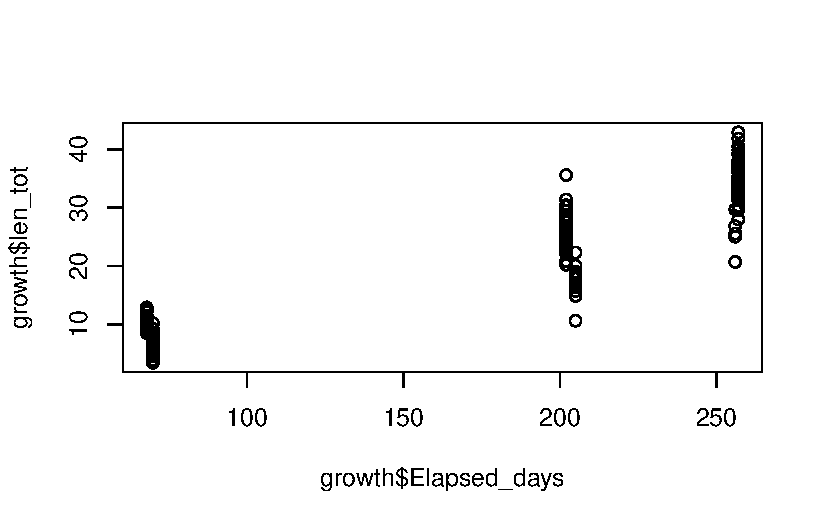
\includegraphics{transplant_growth_lengths_Sep_Dec22_files/figure-pdf/unnamed-chunk-5-1.pdf}

}

\end{figure}

\begin{Shaded}
\begin{Highlighting}[]
\NormalTok{gg2 }\OtherTok{\textless{}{-}} \FunctionTok{ggplot}\NormalTok{(}\AttributeTok{data =}\NormalTok{ growth\_dec, }\FunctionTok{aes}\NormalTok{(}\AttributeTok{x=}\NormalTok{Site, }\AttributeTok{y=}\NormalTok{height\_tot}\SpecialCharTok{/}\NormalTok{Elapsed\_days}\SpecialCharTok{*}\DecValTok{30}\NormalTok{, }\AttributeTok{color =}\NormalTok{ Treatment))}\SpecialCharTok{+}
  \FunctionTok{geom\_boxplot}\NormalTok{()}\SpecialCharTok{+}
  \FunctionTok{xlab}\NormalTok{(}\StringTok{"Site"}\NormalTok{) }\SpecialCharTok{+} 
  \FunctionTok{ylab}\NormalTok{(}\StringTok{"Growth per month (mm)"}\NormalTok{)}\SpecialCharTok{+}
  \FunctionTok{ylim}\NormalTok{(}\DecValTok{0}\NormalTok{,}\DecValTok{9}\NormalTok{)}\SpecialCharTok{+}
  \FunctionTok{scale\_color\_discrete}\NormalTok{(}\AttributeTok{name=}\StringTok{"Shell hash addition"}\NormalTok{)}\SpecialCharTok{+}
  \FunctionTok{ggtitle}\NormalTok{ (}\StringTok{\textquotesingle{}Change in height Sep {-} Dec\textquotesingle{}}\NormalTok{)}

\NormalTok{gg2}
\end{Highlighting}
\end{Shaded}

\begin{verbatim}
Warning: Removed 92 rows containing non-finite values (stat_boxplot).
\end{verbatim}

\begin{figure}[H]

{\centering 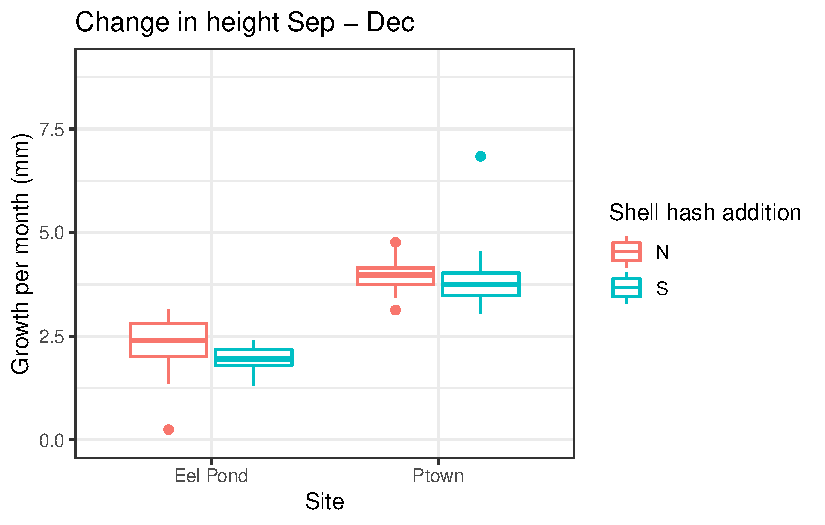
\includegraphics{transplant_growth_lengths_Sep_Dec22_files/figure-pdf/unnamed-chunk-5-2.pdf}

}

\end{figure}

\begin{Shaded}
\begin{Highlighting}[]
\FunctionTok{ggarrange}\NormalTok{(gg1,gg2, }\AttributeTok{ncol=}\DecValTok{2}\NormalTok{, }\AttributeTok{common.legend =} \ConstantTok{TRUE}\NormalTok{, }\AttributeTok{legend =} \StringTok{"right"}\NormalTok{)}
\end{Highlighting}
\end{Shaded}

\begin{verbatim}
Warning: Removed 92 rows containing non-finite values (stat_boxplot).
Removed 92 rows containing non-finite values (stat_boxplot).
Removed 92 rows containing non-finite values (stat_boxplot).
\end{verbatim}

\begin{figure}[H]

{\centering 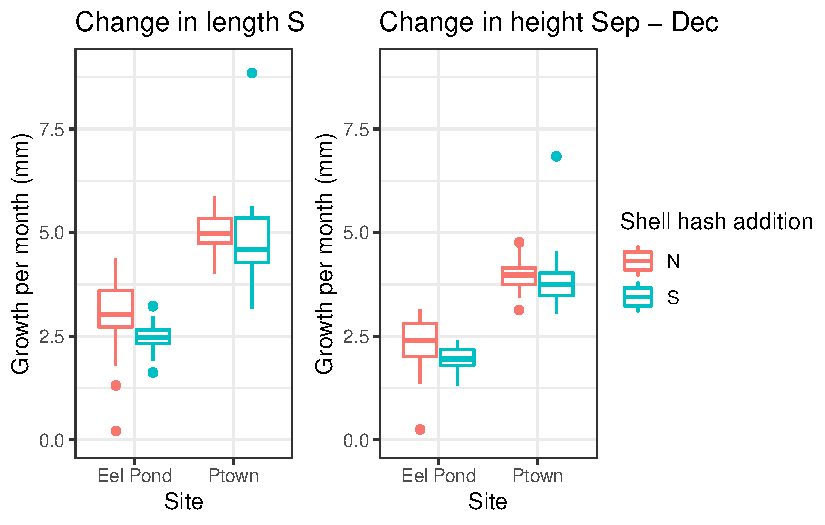
\includegraphics{transplant_growth_lengths_Sep_Dec22_files/figure-pdf/unnamed-chunk-5-3.pdf}

}

\end{figure}

\begin{Shaded}
\begin{Highlighting}[]
\CommentTok{\#{-}{-}{-}{-}{-}{-}{-}{-}{-}{-} Plot for proposal}
\CommentTok{\# Pool treatments}
\NormalTok{gg1 }\OtherTok{\textless{}{-}} \FunctionTok{ggplot}\NormalTok{(}\AttributeTok{data =}\NormalTok{ growth\_dec, }\FunctionTok{aes}\NormalTok{(}\AttributeTok{x=}\NormalTok{Site, }\AttributeTok{y=}\NormalTok{len\_tot}\SpecialCharTok{/}\NormalTok{Elapsed\_days))}\SpecialCharTok{+}
  \FunctionTok{geom\_boxplot}\NormalTok{()}\SpecialCharTok{+}
  \FunctionTok{xlab}\NormalTok{(}\StringTok{"Site"}\NormalTok{) }\SpecialCharTok{+} 
  \FunctionTok{ylab}\NormalTok{(}\StringTok{"Growth (mm/day)"}\NormalTok{)}\SpecialCharTok{+}
  \FunctionTok{ylim}\NormalTok{(}\DecValTok{0}\NormalTok{,}\DecValTok{9}\SpecialCharTok{/}\DecValTok{30}\NormalTok{)}\SpecialCharTok{+}
  \CommentTok{\#scale\_color\_discrete(name="Shell hash addition")+}
  \FunctionTok{ggtitle}\NormalTok{ (}\StringTok{\textquotesingle{}Change in length Sep {-} Dec\textquotesingle{}}\NormalTok{)}
\NormalTok{gg1}
\end{Highlighting}
\end{Shaded}

\begin{verbatim}
Warning: Removed 92 rows containing non-finite values (stat_boxplot).
\end{verbatim}

\begin{figure}[H]

{\centering 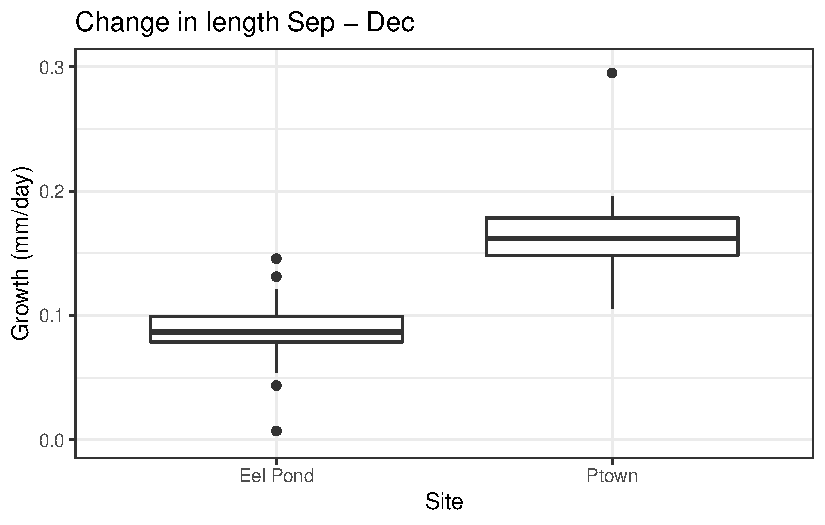
\includegraphics{transplant_growth_lengths_Sep_Dec22_files/figure-pdf/unnamed-chunk-6-1.pdf}

}

\end{figure}

\begin{Shaded}
\begin{Highlighting}[]
\FunctionTok{str}\NormalTok{(growth\_dec)}
\end{Highlighting}
\end{Shaded}

\begin{verbatim}
'data.frame':   188 obs. of  29 variables:
 $ Start_date               : chr  "9/26/2022" "9/26/2022" "9/26/2022" "9/26/2022" ...
 $ Site                     : Factor w/ 2 levels "Eel Pond","Ptown": 1 1 1 1 1 1 1 1 1 1 ...
 $ Treatment                : Factor w/ 2 levels "N","S": 2 2 2 2 2 2 2 2 2 2 ...
 $ Buried_Dec               : chr  "N" "N" "N" "N" ...
 $ Location_code            : chr  "B1" "B1" "B1" "B1" ...
 $ color.1                  : chr  "R" "Y" "B" "L" ...
 $ color.2                  : chr  "" "" "" "" ...
 $ X                        : logi  NA NA NA NA NA NA ...
 $ Start_len_mm             : num  18.2 12.7 12.8 11.2 10.6 ...
 $ Start_height_mm          : num  14 9.63 9.09 8.83 8.21 ...
 $ Start_thickness_mm       : num  8.1 5.56 4.92 4.91 4.42 ...
 $ Collection.month         : chr  "December" "December" "December" "December" ...
 $ Collection1_date         : chr  "12/5/2022" "12/5/2022" "12/5/2022" "12/5/2022" ...
 $ Elapsed_days             : int  70 70 70 70 70 70 70 70 70 70 ...
 $ depth_cm                 : chr  "4+" "" "4+" "" ...
 $ color                    : chr  "R" "" "B" "" ...
 $ L_mm                     : num  NA NA NA NA NA NA NA NA NA NA ...
 $ H_mm                     : num  NA NA NA NA NA NA NA NA NA NA ...
 $ T_mm                     : num  NA NA NA NA NA NA NA NA NA NA ...
 $ growth_marking           : num  10.1 NA NA NA NA NA NA NA NA 7.67 ...
 $ Dead_lengths_mm          : num  18.1 NA NA NA NA ...
 $ growth_height            : num  NA NA NA NA NA NA NA NA NA NA ...
 $ growth_marking_perc_error: num  NA NA NA NA NA NA NA NA NA NA ...
 $ notes                    : chr  "" "" "" "" ...
 $ AliveOrDead              : Factor w/ 3 levels "Alive","Dead",..: 2 3 3 3 3 3 3 3 3 2 ...
 $ len_tot                  : num  NA NA NA NA NA NA NA NA NA NA ...
 $ len_per_day              : num  NA NA NA NA NA NA NA NA NA NA ...
 $ height_tot               : num  NA NA NA NA NA NA NA NA NA NA ...
 $ height_per_day           : num  NA NA NA NA NA NA NA NA NA NA ...
\end{verbatim}

\begin{Shaded}
\begin{Highlighting}[]
\NormalTok{mod\_growth\_full }\OtherTok{\textless{}{-}} \FunctionTok{lme}\NormalTok{(height\_tot}\SpecialCharTok{\textasciitilde{}}\NormalTok{Site}\SpecialCharTok{+}\NormalTok{Start\_len\_mm}\SpecialCharTok{+}\NormalTok{Start\_len\_mm}\SpecialCharTok{:}\NormalTok{Site, }
                       \AttributeTok{random =} \SpecialCharTok{\textasciitilde{}}\DecValTok{1}\SpecialCharTok{|}\NormalTok{Location\_code, }\AttributeTok{data =}\NormalTok{ growth\_dec\_no\_na)}
\FunctionTok{summary}\NormalTok{(mod\_growth\_full)}
\end{Highlighting}
\end{Shaded}

\begin{verbatim}
Linear mixed-effects model fit by REML
  Data: growth_dec_no_na 
       AIC      BIC    logLik
  330.6881 345.8189 -159.3441

Random effects:
 Formula: ~1 | Location_code
        (Intercept) Residual
StdDev:   0.4093236 1.206001

Fixed effects:  height_tot ~ Site + Start_len_mm + Start_len_mm:Site 
                           Value Std.Error DF    t-value p-value
(Intercept)             4.195334 1.8210051 80  2.3038566  0.0238
SitePtown               5.203485 2.2221882 80  2.3416040  0.0217
Start_len_mm            0.055648 0.1569933 80  0.3544640  0.7239
SitePtown:Start_len_mm -0.105721 0.1933691 80 -0.5467292  0.5861
 Correlation: 
                       (Intr) StPtwn Strt__
SitePtown              -0.821              
Start_len_mm           -0.991  0.816       
SitePtown:Start_len_mm  0.804 -0.991 -0.811

Standardized Within-Group Residuals:
        Min          Q1         Med          Q3         Max 
-3.08541873 -0.44802456 -0.05334129  0.43730873  5.22228314 

Number of Observations: 96
Number of Groups: 13 
\end{verbatim}

\begin{Shaded}
\begin{Highlighting}[]
\NormalTok{M\_int}\OtherTok{\textless{}{-}}\FunctionTok{update}\NormalTok{(mod\_growth\_full, .}\SpecialCharTok{\textasciitilde{}}\NormalTok{. }\SpecialCharTok{{-}}\NormalTok{ Start\_len\_mm}\SpecialCharTok{:}\NormalTok{Site)}
\NormalTok{M2 }\OtherTok{\textless{}{-}} \FunctionTok{update}\NormalTok{(M\_int, }\SpecialCharTok{\textasciitilde{}}\NormalTok{. }\SpecialCharTok{{-}}\NormalTok{ Start\_len\_mm)}
\FunctionTok{summary}\NormalTok{(M2)}
\end{Highlighting}
\end{Shaded}

\begin{verbatim}
Linear mixed-effects model fit by REML
  Data: growth_dec_no_na 
       AIC     BIC    logLik
  322.6048 332.778 -157.3024

Random effects:
 Formula: ~1 | Location_code
        (Intercept) Residual
StdDev:   0.4171982 1.193305

Fixed effects:  height_tot ~ Site 
               Value Std.Error DF  t-value p-value
(Intercept) 4.835016 0.2441943 82 19.79987       0
SitePtown   4.006076 0.2869791 82 13.95947       0
 Correlation: 
          (Intr)
SitePtown -0.698

Standardized Within-Group Residuals:
        Min          Q1         Med          Q3         Max 
-3.17505039 -0.50956236 -0.08305134  0.46422437  5.27256861 

Number of Observations: 96
Number of Groups: 13 
\end{verbatim}

\begin{Shaded}
\begin{Highlighting}[]
\NormalTok{(P }\OtherTok{\textless{}{-}} \FunctionTok{mean}\NormalTok{(growth\_dec\_no\_na}\SpecialCharTok{$}\NormalTok{len\_per\_day[growth\_dec\_no\_na}\SpecialCharTok{$}\NormalTok{Site}\SpecialCharTok{==}\StringTok{"Ptown"}\NormalTok{]))}
\end{Highlighting}
\end{Shaded}

\begin{verbatim}
[1] 0.1629378
\end{verbatim}

\begin{Shaded}
\begin{Highlighting}[]
\NormalTok{(E }\OtherTok{\textless{}{-}} \FunctionTok{mean}\NormalTok{(growth\_dec\_no\_na}\SpecialCharTok{$}\NormalTok{len\_per\_day[growth\_dec\_no\_na}\SpecialCharTok{$}\NormalTok{Site}\SpecialCharTok{==}\StringTok{"Eel Pond"}\NormalTok{]))}
\end{Highlighting}
\end{Shaded}

\begin{verbatim}
[1] 0.08792174
\end{verbatim}

\begin{Shaded}
\begin{Highlighting}[]
\NormalTok{E}\SpecialCharTok{/}\NormalTok{P}
\end{Highlighting}
\end{Shaded}

\begin{verbatim}
[1] 0.5396029
\end{verbatim}

\begin{Shaded}
\begin{Highlighting}[]
\NormalTok{(P}\SpecialCharTok{{-}}\NormalTok{E)}\SpecialCharTok{/}\NormalTok{E}
\end{Highlighting}
\end{Shaded}

\begin{verbatim}
[1] 0.8532145
\end{verbatim}

\begin{Shaded}
\begin{Highlighting}[]
\NormalTok{P}\SpecialCharTok{/}\NormalTok{E}
\end{Highlighting}
\end{Shaded}

\begin{verbatim}
[1] 1.853215
\end{verbatim}

\begin{Shaded}
\begin{Highlighting}[]
\NormalTok{Alive\_count }\OtherTok{\textless{}{-}}\NormalTok{ growth\_dec }\SpecialCharTok{\%\textgreater{}\%} \FunctionTok{count}\NormalTok{(Treatment, Site, Location\_code, AliveOrDead)}
\NormalTok{mod\_growth\_full }\OtherTok{\textless{}{-}} \FunctionTok{lme}\NormalTok{(n}\SpecialCharTok{\textasciitilde{}}\NormalTok{Treatment}\SpecialCharTok{*}\NormalTok{Site, }
                       \AttributeTok{random =} \SpecialCharTok{\textasciitilde{}}\DecValTok{1}\SpecialCharTok{|}\NormalTok{Location\_code, }\AttributeTok{data =}\NormalTok{ Alive\_count)}
\FunctionTok{summary}\NormalTok{(mod\_growth\_full) }\CommentTok{\# Not really answering my question but not differences in survival between treatments}
\end{Highlighting}
\end{Shaded}

\begin{verbatim}
Linear mixed-effects model fit by REML
  Data: Alive_count 
       AIC      BIC   logLik
  199.8378 209.3389 -93.9189

Random effects:
 Formula: ~1 | Location_code
         (Intercept) Residual
StdDev: 0.0004674892 2.894189

Fixed effects:  n ~ Treatment * Site 
                         Value Std.Error DF   t-value p-value
(Intercept)           4.750000  1.023251 24  4.642069  0.0001
TreatmentS           -0.194444  1.406323 24 -0.138264  0.8912
SitePtown             0.159091  1.344815 24  0.118300  0.9068
TreatmentS:SitePtown -0.131313  1.853984 24 -0.070828  0.9441
 Correlation: 
                     (Intr) TrtmnS StPtwn
TreatmentS           -0.728              
SitePtown            -0.761  0.554       
TreatmentS:SitePtown  0.552 -0.759 -0.725

Standardized Within-Group Residuals:
       Min         Q1        Med         Q3        Max 
-1.3506686 -0.7154704 -0.2303466  0.7918164  2.4500500 

Number of Observations: 40
Number of Groups: 13 
\end{verbatim}

\begin{Shaded}
\begin{Highlighting}[]
\FunctionTok{library}\NormalTok{(lme4)}
\end{Highlighting}
\end{Shaded}

\begin{verbatim}
Loading required package: Matrix
\end{verbatim}

\begin{verbatim}

Attaching package: 'lme4'
\end{verbatim}

\begin{verbatim}
The following object is masked from 'package:nlme':

    lmList
\end{verbatim}

\begin{Shaded}
\begin{Highlighting}[]
\NormalTok{growth\_dec}\SpecialCharTok{$}\NormalTok{AliveOrDead}
\end{Highlighting}
\end{Shaded}

\begin{verbatim}
  [1] Dead    Missing Missing Missing Missing Missing Missing Missing Missing
 [10] Dead    Alive   Alive   Alive   Dead    Dead    Alive   Alive   Missing
 [19] Alive   Dead    Missing Alive   Missing Missing Missing Dead    Dead   
 [28] Missing Missing Alive   Missing Alive   Alive   Dead    Dead    Alive  
 [37] Alive   Alive   Alive   Missing Missing Alive   Alive   Alive   Alive  
 [46] Alive   Missing Missing Missing Missing Alive   Missing Alive   Alive  
 [55] Alive   Alive   Alive   Alive   Dead    Missing Missing Missing Alive  
 [64] Alive   Missing Alive   Alive   Dead    Dead    Dead    Alive   Alive  
 [73] Alive   Alive   Alive   Alive   Alive   Alive   Alive   Alive   Missing
 [82] Missing Missing Missing Missing Missing Missing Missing Alive   Alive  
 [91] Dead    Missing Missing Missing Missing Missing Missing Alive   Alive  
[100] Dead    Dead    Alive   Missing Alive   Alive   Alive   Alive   Alive  
[109] Alive   Dead    Alive   Alive   Missing Alive   Missing Missing Missing
[118] Alive   Alive   Alive   Dead    Alive   Alive   Alive   Missing Missing
[127] Missing Missing Missing Missing Alive   Alive   Alive   Alive   Missing
[136] Alive   Alive   Missing Missing Dead    Alive   Alive   Alive   Alive  
[145] Alive   Alive   Dead    Alive   Alive   Alive   Alive   Dead    Alive  
[154] Missing Alive   Dead    Alive   Alive   Missing Alive   Missing Alive  
[163] Alive   Alive   Alive   Alive   Alive   Alive   Alive   Alive   Alive  
[172] Alive   Alive   Alive   Alive   Alive   Missing Missing Missing Missing
[181] Missing Missing Missing Missing Missing Missing Missing Missing
Levels: Alive Dead Missing
\end{verbatim}

\begin{Shaded}
\begin{Highlighting}[]
\NormalTok{(gm1 }\OtherTok{\textless{}{-}} \FunctionTok{glmer}\NormalTok{(AliveOrDead }\SpecialCharTok{\textasciitilde{}}\NormalTok{ Treatment }\SpecialCharTok{*}\NormalTok{Site }\SpecialCharTok{+}\NormalTok{ (}\DecValTok{1} \SpecialCharTok{|}\NormalTok{ Location\_code),}
              \AttributeTok{data =}\NormalTok{ growth\_dec, }\AttributeTok{family =}\NormalTok{ binomial))}
\end{Highlighting}
\end{Shaded}

\begin{verbatim}
Generalized linear mixed model fit by maximum likelihood (Laplace
  Approximation) [glmerMod]
 Family: binomial  ( logit )
Formula: AliveOrDead ~ Treatment * Site + (1 | Location_code)
   Data: growth_dec
      AIC       BIC    logLik  deviance  df.resid 
 253.5739  269.7562 -121.7870  243.5739       183 
Random effects:
 Groups        Name        Std.Dev.
 Location_code (Intercept) 1.098   
Number of obs: 188, groups:  Location_code, 13
Fixed Effects:
         (Intercept)            TreatmentS             SitePtown  
              1.0258               -2.0117               -0.2452  
TreatmentS:SitePtown  
              0.3584  
\end{verbatim}

\begin{Shaded}
\begin{Highlighting}[]
\FunctionTok{summary}\NormalTok{(gm1) }\CommentTok{\#Here there is an effect of treatment but it\textquotesingle{}s still not answering my question about initial lengths}
\end{Highlighting}
\end{Shaded}

\begin{verbatim}
Generalized linear mixed model fit by maximum likelihood (Laplace
  Approximation) [glmerMod]
 Family: binomial  ( logit )
Formula: AliveOrDead ~ Treatment * Site + (1 | Location_code)
   Data: growth_dec

     AIC      BIC   logLik deviance df.resid 
   253.6    269.8   -121.8    243.6      183 

Scaled residuals: 
    Min      1Q  Median      3Q     Max 
-1.8107 -0.8039 -0.3536  0.8054  2.3304 

Random effects:
 Groups        Name        Variance Std.Dev.
 Location_code (Intercept) 1.206    1.098   
Number of obs: 188, groups:  Location_code, 13

Fixed effects:
                     Estimate Std. Error z value Pr(>|z|)  
(Intercept)            1.0258     0.7015   1.462   0.1437  
TreatmentS            -2.0117     0.9474  -2.123   0.0337 *
SitePtown             -0.2452     0.6906  -0.355   0.7225  
TreatmentS:SitePtown   0.3584     0.9780   0.366   0.7140  
---
Signif. codes:  0 '***' 0.001 '**' 0.01 '*' 0.05 '.' 0.1 ' ' 1

Correlation of Fixed Effects:
            (Intr) TrtmnS StPtwn
TreatmentS  -0.780              
SitePtown   -0.710  0.666       
TrtmntS:StP  0.460 -0.661 -0.767
\end{verbatim}

\begin{Shaded}
\begin{Highlighting}[]
\NormalTok{growth\_dec}\SpecialCharTok{$}\NormalTok{Start\_len\_mm}
\end{Highlighting}
\end{Shaded}

\begin{verbatim}
  [1] 18.21000 12.71000 12.80000 11.23000 10.59000  9.94000 10.11000  9.03000
  [9] 10.08000 10.52714 10.52714 10.52714 10.52714 14.34000 13.25000 13.53000
 [17] 12.80000 11.27000 11.03000 10.97000 10.72000  9.88000 11.97667 15.10000
 [25] 13.60000 12.80000 12.00000 11.70000  9.90000  9.80000 10.80000 11.40000
 [33] 11.90000 11.90000 11.90000 14.20000 13.30000 11.70000 12.30000 10.80000
 [41]  9.80000  9.70000 11.10000 10.00000 12.60000 13.20000 10.90000 11.60000
 [49] 12.20000 10.20000 11.80000 10.90000 11.10000 11.61111 11.61111 11.61111
 [57] 14.50000 11.40000 11.90000 11.70000 11.20000 10.60000  9.60000 11.40000
 [65] 10.70000 11.44444 11.44444 11.44444 11.44444 11.44444 13.50000 12.10000
 [73] 11.50000 11.30000 10.20000  9.40000 10.10000 11.00000 11.50000 13.83000
 [81] 12.84000 11.78000 11.25000 10.27000  9.95000 10.11000  9.67000  8.94000
 [89] 10.60125 13.98000 11.54000 11.51000 11.30000 10.72000  9.28000 10.24000
 [97]  9.88000  8.76000 10.48833 12.94000 11.89000 11.93000 11.02000 10.45000
[105] 10.32000 10.12000  9.75000  8.98000 10.82222 10.82222 12.98000 12.69000
[113] 11.80000 11.51000 11.38000  9.95000 10.02000  9.48000  9.47000 11.03111
[121] 11.03111 12.15000 10.41000 11.23000 10.94000 10.96000 11.12000  8.63000
[129]  9.69000  9.33000 10.11167 10.11167 10.11167 10.11167 10.11167 14.30000
[137] 12.10000 12.20000 11.30000 11.00000 11.70000 10.40000 10.00000  8.90000
[145] 11.32222 11.32222 14.00000 13.30000 11.90000 11.40000 11.20000 10.70000
[153] 10.80000 10.30000  9.80000 10.30000 14.60000 13.10000 11.30000 11.40000
[161] 11.50000 10.00000  9.90000 10.20000  8.70000 11.18889 11.50000 14.70000
[169] 11.30000 11.20000 10.80000 10.80000 10.60000 10.20000 10.30000  9.40000
[177] 12.90000 12.30000 12.90000 11.40000 10.60000  9.80000 10.10000 10.80000
[185]  8.80000 11.06667 11.06667 11.06667
\end{verbatim}

\begin{Shaded}
\begin{Highlighting}[]
\NormalTok{(gm1 }\OtherTok{\textless{}{-}} \FunctionTok{lme}\NormalTok{(Start\_len\_mm }\SpecialCharTok{\textasciitilde{}}\NormalTok{ Treatment }\SpecialCharTok{*}\NormalTok{AliveOrDead}\SpecialCharTok{+}\NormalTok{ Site, }
            \AttributeTok{random =} \SpecialCharTok{\textasciitilde{}}\DecValTok{1} \SpecialCharTok{|}\NormalTok{ Location\_code,}
              \AttributeTok{data =}\NormalTok{ growth\_dec))}
\end{Highlighting}
\end{Shaded}

\begin{verbatim}
Linear mixed-effects model fit by REML
  Data: growth_dec 
  Log-restricted-likelihood: -320.42
  Fixed: Start_len_mm ~ Treatment * AliveOrDead + Site 
                  (Intercept)                    TreatmentS 
                   11.6049490                    -0.1376432 
              AliveOrDeadDead            AliveOrDeadMissing 
                    0.4294367                    -0.1624917 
                    SitePtown    TreatmentS:AliveOrDeadDead 
                   -0.4993074                     0.8990295 
TreatmentS:AliveOrDeadMissing 
                   -0.3390275 

Random effects:
 Formula: ~1 | Location_code
        (Intercept) Residual
StdDev: 4.55376e-05 1.332229

Number of Observations: 188
Number of Groups: 13 
\end{verbatim}

\begin{Shaded}
\begin{Highlighting}[]
\FunctionTok{summary}\NormalTok{(gm1)}
\end{Highlighting}
\end{Shaded}

\begin{verbatim}
Linear mixed-effects model fit by REML
  Data: growth_dec 
       AIC      BIC  logLik
  658.8399 687.6264 -320.42

Random effects:
 Formula: ~1 | Location_code
        (Intercept) Residual
StdDev: 4.55376e-05 1.332229

Fixed effects:  Start_len_mm ~ Treatment * AliveOrDead + Site 
                                  Value Std.Error  DF  t-value p-value
(Intercept)                   11.604949 0.2419998 169 47.95438  0.0000
TreatmentS                    -0.137643 0.2758059 169 -0.49906  0.6184
AliveOrDeadDead                0.429437 0.4150945 169  1.03455  0.3024
AliveOrDeadMissing            -0.162492 0.3018549 169 -0.53831  0.5911
SitePtown                     -0.499307 0.1985573 169 -2.51468  0.0128
TreatmentS:AliveOrDeadDead     0.899029 0.6517401 169  1.37943  0.1696
TreatmentS:AliveOrDeadMissing -0.339027 0.4222122 169 -0.80298  0.4231
 Correlation: 
                              (Intr) TrtmnS AlvODD AlvODM StPtwn TS:AODD
TreatmentS                    -0.669                                    
AliveOrDeadDead               -0.482  0.388                             
AliveOrDeadMissing            -0.597  0.533  0.352                      
SitePtown                     -0.492  0.008  0.082 -0.021               
TreatmentS:AliveOrDeadDead     0.275 -0.423 -0.632 -0.226  0.013        
TreatmentS:AliveOrDeadMissing  0.428 -0.653 -0.252 -0.715  0.013  0.277 

Standardized Within-Group Residuals:
       Min         Q1        Med         Q3        Max 
-1.8057262 -0.6427810 -0.1258433  0.4322162  4.0640357 

Number of Observations: 188
Number of Groups: 13 
\end{verbatim}

\begin{Shaded}
\begin{Highlighting}[]
\CommentTok{\#growth\_dec$AliveOrDead[growth\_dec$AliveOrDead=="Missing"]\textless{}{-} NA}
\CommentTok{\# p \textless{}{-} ggplot(growth\_dec, aes(x = Treatment, y = Start\_len\_mm, }
\CommentTok{\#                             color = AliveOrDead))}
\CommentTok{\# p + geom\_boxplot() + facet\_grid(Site \textasciitilde{} .)}
\CommentTok{\# }
\CommentTok{\# p \textless{}{-} ggplot(growth\_dec, aes(x = Start\_len\_mm, y = AliveOrDead, }
\CommentTok{\#                             color = Treatment))}
\CommentTok{\# p + geom\_boxplot() + facet\_grid(Site \textasciitilde{} .)}
\end{Highlighting}
\end{Shaded}

\begin{Shaded}
\begin{Highlighting}[]
\NormalTok{Alive }\OtherTok{\textless{}{-}} \FunctionTok{as.data.frame}\NormalTok{(Alive\_count[Alive\_count}\SpecialCharTok{$}\NormalTok{AliveOrDead}\SpecialCharTok{==}\StringTok{"Alive"}\NormalTok{,])}
\NormalTok{Alive}\SpecialCharTok{$}\NormalTok{perc\_alive }\OtherTok{\textless{}{-}}\NormalTok{ Alive}\SpecialCharTok{$}\NormalTok{n}\SpecialCharTok{/}\DecValTok{9}\SpecialCharTok{*}\DecValTok{100}
\NormalTok{Alive}
\end{Highlighting}
\end{Shaded}

\begin{verbatim}
   Treatment     Site Location_code AliveOrDead n perc_alive
1          N Eel Pond            F1       Alive 3   33.33333
4          N Eel Pond            H2       Alive 7   77.77778
6          N Eel Pond            I3       Alive 6   66.66667
9          N    Ptown            A2       Alive 2   22.22222
11         N    Ptown            C3       Alive 7   77.77778
14         N    Ptown            G2       Alive 6   66.66667
17         N    Ptown            H2       Alive 9  100.00000
20         S Eel Pond            B1       Alive 3   33.33333
23         S Eel Pond            E2       Alive 4   44.44444
26         S Eel Pond            G2       Alive 7   77.77778
28         S Eel Pond            J3       Alive 9  100.00000
29         S    Ptown            B3       Alive 3   33.33333
32         S    Ptown            D2       Alive 6   66.66667
35         S    Ptown            E2       Alive 7   77.77778
37         S    Ptown            F3       Alive 8   88.88889
40         S    Ptown            I4       Alive 9  100.00000
\end{verbatim}



\end{document}
